\documentclass[11pt]{article}
\usepackage[margin=1in]{geometry}

% Times (Times New Roman look-alike, works with pdfLaTeX)
\usepackage[T1]{fontenc}
\usepackage{mathptmx}

% Core packages
\usepackage{amsmath,amssymb}
\usepackage{multicol}
\usepackage{graphicx}
\usepackage{fancyhdr}

% Tables, floats, colour, charts
\usepackage[table]{xcolor}
\usepackage{booktabs,tabularx,array,float,enumitem}
\usepackage[font=small,labelfont=bf,skip=4pt]{caption}
\usepackage{tikz}
\usetikzlibrary{arrows.meta,positioning,calc,fit,backgrounds}
\usepackage{pgfplots}
\pgfplotsset{compat=1.16}
\usepackage[colorlinks=true,linkcolor=black,citecolor=black,urlcolor=blue]{hyperref}
\usepackage{lastpage}
\usepackage{titlesec}
\usepackage{tocloft}

% Thin black border for every figure and table
\setlength{\fboxrule}{0.4pt}
\setlength{\fboxsep}{5pt}

\definecolor{accent}{RGB}{37,99,235}
\definecolor{barmuted}{RGB}{196,196,184}
\definecolor{darkgrey}{RGB}{80,80,80}
\definecolor{okgreen}{RGB}{22,128,70}
\definecolor{warnred}{RGB}{190,40,40}

% Tighter spacing for headings, floats and contents
\titlespacing*{\section}{0pt}{9pt plus 2pt minus 2pt}{3pt plus 1pt}
\titlespacing*{\subsection}{0pt}{6pt plus 2pt minus 2pt}{2pt plus 1pt}
\setlength{\intextsep}{6pt plus 2pt minus 2pt}
\setlength{\floatsep}{6pt plus 2pt minus 2pt}
\setlength{\textfloatsep}{6pt plus 2pt minus 2pt}
\setlength{\abovedisplayskip}{4pt plus 1pt minus 1pt}
\setlength{\belowdisplayskip}{4pt plus 1pt minus 1pt}
\setlength{\cftbeforesecskip}{2pt}
\setlength{\cftbeforesubsecskip}{0pt}
\setlength{\cftbeforefigskip}{1pt}
\setlength{\cftbeforetabskip}{1pt}
\setlength{\cfttabnumwidth}{2.4em}
\emergencystretch=2em

% Paragraphs
\setlength{\parindent}{0pt}
\setlength{\parskip}{0.3\baselineskip plus 1pt}
\setlist{itemsep=1pt,topsep=1pt,parsep=0pt}
\renewcommand{\arraystretch}{1.28}

% Project details (cover page)
\newcommand{\ProjectTitle}{Edge-to-Server Dual-Mode CCTV Anomaly Detection with Agentic Triage: Home Security and Public Space Monitoring}
\newcommand{\ShortTitle}{Dual-Mode CCTV Anomaly Detection}
\newcommand{\ReportType}{Project Report}
\newcommand{\StudentName}{R. Ganesh}
\newcommand{\RegisterNumber}{RA2212704010031}
\newcommand{\FacultyName}{Dr. S. Aswath}
\newcommand{\FacultyRole}{Assistant Professor}
\newcommand{\CourseCode}{21AIE535T}
\newcommand{\CourseName}{Artificial Intelligence and Internet of Things}
\newcommand{\DepartmentName}{Department of Data Science and Business Systems}

% Header and footer: used on every page except the first (title page)
\setlength{\headheight}{14pt}
\newcommand{\HFstyle}{%
  \fancyhf{}%
  \fancyhead[L]{\small\itshape \ShortTitle}%
  \fancyhead[R]{\small \CourseCode}%
  \fancyfoot[L]{\small \StudentName\ [\RegisterNumber]}%
  \fancyfoot[R]{\small \thepage/\pageref{LastPage}}%
  \renewcommand{\headrulewidth}{0.4pt}%
  \renewcommand{\footrulewidth}{0.4pt}}
\pagestyle{fancy}
\HFstyle
\fancypagestyle{plain}{\HFstyle}

% Helpers
\newcolumntype{Y}{>{\raggedright\arraybackslash}X}
\newcolumntype{L}[1]{>{\raggedright\arraybackslash}p{#1}}
\DeclareRobustCommand{\code}[1]{\texttt{\detokenize{#1}}}
\newcommand{\TW}{\dimexpr\textwidth-2\fboxsep-2\fboxrule\relax}

% Matrix cell shortcuts
\newcommand{\Yes}{\cellcolor{green!18}Yes}
\newcommand{\No}{\cellcolor{red!15}No}
\newcommand{\Part}{\cellcolor{yellow!25}Partial}

\begin{document}

% ---------------- First page: no header, footer or page number ----------------
\begin{titlepage}
\thispagestyle{empty}
\centering
\setlength{\parskip}{0pt}
\vspace*{0.15in}

{\bfseries\MakeUppercase{\ProjectTitle}\par}
\vspace{\stretch{1.1}}

{\MakeUppercase{\ReportType}\par}
\vspace{0.3in}
BY\par
\vspace{\stretch{1}}

{\Large\bfseries \StudentName\par}
\vspace{0.1in}
{\large\bfseries [\RegisterNumber]\par}
\vspace{\stretch{1.1}}

Under the guidance of\par
\vspace{0.12in}
{\Large\bfseries \FacultyName\par}
{\itshape \FacultyRole\par}
{\itshape \DepartmentName\par}
\vspace{\stretch{1}}

{\itshape In partial fulfillment of the course\par}
\vspace{0.2in}
{\bfseries\itshape \CourseCode{} -- \CourseName\par}
\vspace{0.2in}
{\bfseries\itshape in\par}
{\bfseries\itshape Department of Data Science and\par
Business Systems\par}
\vspace{\stretch{1.1}}

\IfFileExists{srm_logo.png}%
  {
\includegraphics[width=2.6in]{srm_logo.png}}%
  {\fbox{\parbox[c][1.6in][c]{2.15in}{\centering Logo placeholder\\[2pt]\small add srm\_logo.png}}}\par
\vspace{0.25in}
{\bfseries FACULTY OF ENGINEERING AND TECHNOLOGY\par}
\vspace{0.2in}
{\bfseries SCHOOL OF COMPUTING\par}
\vspace{0.2in}
{\bfseries SRM INSTITUTE OF SCIENCE AND TECHNOLOGY\par}
\vspace{0.2in}
{\bfseries KATTANKULATHUR\par}
\vspace{\stretch{0.4}}
\end{titlepage}

% ---------------- Contents ----------------
\tableofcontents
\clearpage
\listoffigures
\listoftables
\clearpage

% ---------------- Abstract ----------------
\section*{Abstract}
\addcontentsline{toc}{section}{Abstract}

Commercial smart-home and public CCTV platforms usually treat the camera as a thin sensor and the vendor cloud as the place where detection happens. Raw video leaves the building, the owner pays a recurring fee for the intelligence, and the system stops being useful when the cloud is unreachable. This project builds the opposite: a self-hosted, two-process pipeline in which an \textbf{edge node} (the IoT camera device, simulated for now) captures and compresses frames and a separate \textbf{analysis server} performs all computer vision locally. The server runs a quantised NMS-free \code{YOLO26n} model through ONNX Runtime, tracks objects across frames, and evaluates a comprehensive rule set in two selectable modes, \textbf{Home Security} and \textbf{Public Space}. Every rule hit is passed to a text-only \textbf{LangGraph} triage agent backed by a cloud LLM, which decides whether to alert or suppress; the agent never receives an image and fails open if the model is unreachable. Confirmed alerts are delivered to a phone through the \textbf{Hermes Agent} gateway and \textbf{Telegram}, and two React consoles monitor and control the system.

The two backends run as \textbf{separate servers on separate ports}: the simulated IoT edge node on \code{:8001} and the analysis server on \code{:8000}, joined only by HTTP \code{POST /frames}. Measured on an Intel Core i5-12500H, JPEG edge compression reduces uplink traffic by about 97\% against raw frames, ONNX inference averages 27.6 ms in isolation, all 26 automated tests pass, and an end-to-end live run with the full stack produced real Telegram alerts within seconds of detection. The live run also exposed weaknesses (alert bursts, a tamper false positive at the video loop point, and one LLM timeout handled by fail-open), which are reported and analysed rather than hidden.

\textbf{Key findings}

\begin{table}[H]
\centering\small
\caption{Key findings of the project}
\label{tab:ieee_1}
\begin{tabularx}{\textwidth}{|r|Y|Y|}
\hline
\rowcolor{black!8} \textbf{\#} & \textbf{Finding} & \textbf{Evidence} \\ \hline
1 & Edge and server run as two independent processes joined only by HTTP & Edge \code{:8001}, server \code{:8000}; frames arrive as \code{POST /frames} \\ \hline
2 & JPEG edge encoding removes most of the uplink cost & 23.3--31.0 KB per frame against 900 KB raw ($\approx$97\% less) \\ \hline
3 & Local ONNX inference is fast enough for real time on a laptop CPU & 27.6 ms per frame in isolation (about 36 FPS capacity) \\ \hline
4 & Under full load the pipeline sustained 6.6 FPS with some frame loss & Live run: 2,859 frames received, 102 dropped (3.6\%) \\ \hline
5 & Two operating modes share one detector and tracker & Home (18 rule families) and Public (20 implemented rules), plus shared camera-health rules \\ \hline
6 & Text-only LLM triage works and degrades safely & Reasons attached to alerts; one \code{fail-open} after a timeout \\ \hline
7 & Alerts reach the owner's phone in structured form & Twelve Telegram alert cards in about 19 seconds of one live run \\ \hline
8 & The live run exposed alert noise that needs tuning & Burst of casing/zone alerts, tamper flag at loop restart \\ \hline
9 & Automated verification passes & 26/26 \code{pytest} cases; precision 1.00, recall 1.00 on two self-labelled clips \\ \hline
\end{tabularx}
\end{table}

% ---------------- 1 ----------------
\section{Introduction and Problem Statement}

Closed-circuit television has moved from dedicated control rooms into ordinary homes, shops and public spaces. The camera is now cheap; the intelligence is not. A modern camera is expected to tell the owner what happened (a person at the door, a bag left on a platform) rather than merely record it, and that capability normally depends on a vendor's cloud. This creates three problems for a student of AI and the Internet of Things.

\begin{enumerate}
  \item \textbf{Privacy.} Video of a home or a public concourse is sent to a third party before anyone decides whether it matters.
  \item \textbf{Dependence.} If the vendor's service is unreachable, discontinued or repriced, the camera stops being useful even though the hardware still works.
  \item \textbf{Noise.} Simple motion detection fires on pets, shadows and passers-by, so owners learn to ignore alerts. Better detection is needed, but so is better judgement about which detections deserve an alert.
\end{enumerate}

This project asks whether a small team can build a pipeline that keeps video local, detects objects in real time on ordinary hardware, applies domain-specific rules for two very different settings, and still benefits from the contextual judgement of a large language model without ever sending the LLM a picture.

\textbf{Research questions}
\begin{enumerate}
  \item How should capture and analysis be split so that a resource-constrained IoT camera node and a more powerful server cooperate cleanly over HTTP?
  \item How can one detector and tracker serve both Home Security (zones, night hours, pets, parcels) and Public Space (crowds, unattended baggage, restricted areas)?
  \item Can an LLM reduce false alarms using only text metadata, and what must happen when it is unavailable?
  \item How should confirmed alerts reach the owner reliably on a phone?
  \item What does a live, end-to-end run reveal about accuracy, latency, frame loss and alert quality?
\end{enumerate}

\textbf{Scope and method.} The report describes the implemented system (source code in the \code{edge/}, \code{server/}, \code{frontend/} and \code{tests/} directories of the project), the data acquired for demonstration, the automated tests, an offline evaluation script, and one documented live run on 17 November 2026 using a security-camera clip. Performance figures are measured on a single laptop (Intel Core i5-12500H); figures for the isolated pipeline come from the project benchmark, and figures for the full stack come from the live run screenshots reproduced in Section~\ref{sec:results}.

\subsection{Background: from raw pixels to contextual alerts}

Early rule engines fire directly on raw bounding boxes. That breaks in practice: a brief occlusion drops a track, a dog triggers an intruder alarm, and a one-frame confidence flicker produces an alert storm. This project therefore separates three concerns. A fast detector produces boxes in milliseconds. A tracker and rule engine turn boxes into events using time, geometry and history. A final triage stage uses language-model reasoning on the event description to decide whether the owner should be interrupted. Separating them keeps each stage testable, and it keeps the expensive and privacy-sensitive stage (the LLM) away from the pixels.

\subsection{Key terms}

\begin{table}[H]
\centering\small
\caption{Key terms used in this report}
\label{tab:ieee_2}
\begin{tabularx}{\textwidth}{|L{3.6cm}|Y|}
\hline
\rowcolor{black!8} \textbf{Term} & \textbf{Meaning in this report} \\ \hline
Edge node & The IoT camera-side process that captures frames, resizes and JPEG-encodes them, and posts them to the server \\ \hline
Simulated IoT device & The edge node running as its own process on the laptop, reading video files as if they were a camera, because Raspberry Pi hardware was unavailable \\ \hline
Analysis server & The FastAPI process that runs detection, tracking, rules, triage, storage and alerting \\ \hline
YOLO26n ONNX & A nano object detector exported without non-maximum suppression and run by ONNX Runtime on the CPU \\ \hline
Letterbox & Resizing with grey padding so a frame fits the 640$\times$640 model input without distortion \\ \hline
Hysteresis & A higher confidence to start tracking an object than to keep tracking it, to prevent flicker \\ \hline
Zone & A named polygon in normalised image coordinates (for example \code{door} or \code{restricted}) \\ \hline
Arming state & Home-mode setting (\code{disarmed}, \code{armed_home}, \code{armed_night}, \code{armed_away}) that selects which rules are active \\ \hline
Triage agent & A four-node LangGraph workflow that reads an alert as text and decides to notify or suppress \\ \hline
Fail-open & If the LLM or its network fails, the alert is still sent \\ \hline
Hermes Agent & A local messaging gateway that receives a signed webhook and delivers it to Telegram \\ \hline
\end{tabularx}
\end{table}

% ---------------- 2 ----------------
\section{Project Overview and Objectives}

\subsection{Objectives}

\begin{table}[H]
\centering\small
\caption{Project objectives and how each was addressed}
\label{tab:ieee_3}
\begin{tabularx}{\textwidth}{|r|L{4.4cm}|Y|}
\hline
\rowcolor{black!8} \textbf{\#} & \textbf{Objective} & \textbf{How it was addressed} \\ \hline
O1 & Keep video local & All detection runs on the analysis server with ONNX Runtime; only text metadata reaches the LLM \\ \hline
O2 & Model an IoT device honestly & Edge node built as a separate uvicorn process on its own port with its own control API \\ \hline
O3 & Support two domains & One \code{RuleEngine} with \code{home} and \code{public} modes switchable at run time \\ \hline
O4 & Reduce false alarms & Per-class thresholds, hysteresis, multi-frame confirmation, pet filtering, arming states, LLM triage \\ \hline
O5 & Deliver alerts to a phone & HMAC-signed webhook to Hermes, which posts a formatted card to Telegram \\ \hline
O6 & Make it observable & Two React consoles plus REST endpoints, SQLite event log and frame metrics \\ \hline
O7 & Verify it & 26 automated tests, an offline evaluation script and a documented live run \\ \hline
\end{tabularx}
\end{table}

\subsection{Requirements}

\begin{table}[H]
\centering\small
\caption{Functional and non-functional requirements}
\label{tab:ieee_4}
\begin{tabularx}{\textwidth}{|L{2.0cm}|Y|L{3.3cm}|}
\hline
\rowcolor{black!8} \textbf{Type} & \textbf{Requirement} & \textbf{Verified by} \\ \hline
Functional & Accept JPEG frames over HTTP with a device id, timestamp and sequence number & \code{POST /frames} tests \\ \hline
Functional & Detect people, vehicles, bags and pets with bounding boxes & Annotated feed in console \\ \hline
Functional & Evaluate zone, time, count and dwell rules in two modes & Rule unit tests \\ \hline
Functional & Switch mode and arming without a restart & \code{GET/POST /mode} \\ \hline
Functional & Send an alert card to Telegram & Live run screenshots \\ \hline
Non-functional & Never block the frame loop on the LLM & Background executor \\ \hline
Non-functional & Never lose an alert because a cloud is down & Fail-open test \\ \hline
Non-functional & Reject oversized or malformed uploads & Security tests (413, 400, 401, 403) \\ \hline
Non-functional & Keep the video off the public internet & Local-only ports, text-only agent \\ \hline
\end{tabularx}
\end{table}

\subsection{Assumptions and constraints}

\begin{itemize}
  \item Raspberry Pi hardware was unavailable, so the IoT camera node is \textbf{simulated} as a separate process that reads video files; the code is written so the same process could run on a Raspberry Pi 4 with a USB webcam, but this has not been tested on hardware.
  \item The detector is a COCO-80 model. It cannot see parcels, faces, fire or pose, so rules that need those are out of scope (Section~\ref{sec:limits}).
  \item The server, edge simulator, two web consoles and the Hermes gateway all run on one laptop for the demonstration; the LLM is the only cloud dependency.
\end{itemize}

% ---------------- 3 ----------------
\section{System Architecture}

The system is divided into independent processes that talk only over HTTP (Fig.~\ref{fig:topology}). The simulated IoT edge node and the analysis server are \textbf{two separate servers on two separate ports}. Neither imports the other's state at run time; the edge node simply posts frames to the server, and the web consoles talk to whichever backend owns the function they control.

\begin{figure}[H]
\centering
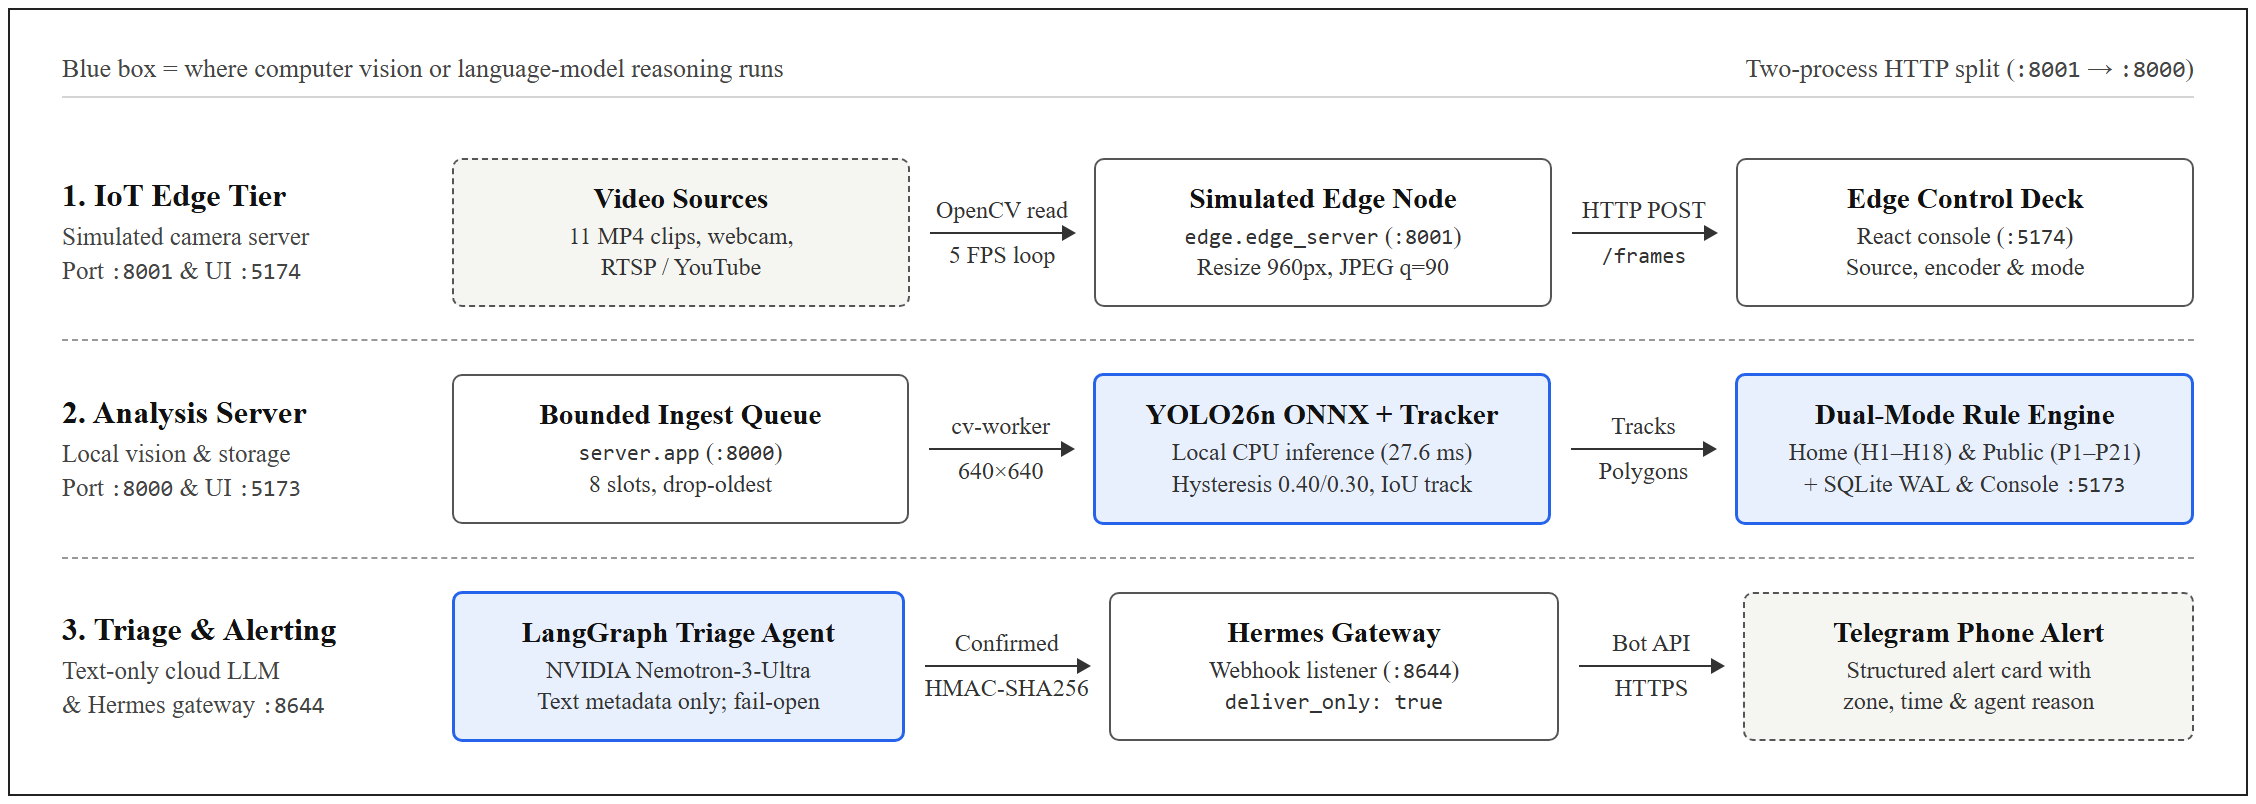
\includegraphics[width=0.98\linewidth]{figures/fig1_topology.png}
\caption{Two-server deployment topology rendered from HTML architecture specification. The simulated IoT edge node (\code{:8001}) and the analysis server (\code{:8000}) run as independent OS processes communicating over HTTP \code{POST /frames}; raw frames never reach the cloud LLM.}
\label{fig:topology}
\end{figure}

\subsection{Processes, ports and responsibilities}

Table~\ref{tab:procs} summarises the five runtime processes that form the complete system and the network port assigned to each service.

\begin{table}[H]
\centering\small
\caption{Every process in the running system}
\label{tab:procs}
\begin{tabularx}{\textwidth}{|L{3.1cm}|L{1.2cm}|L{3.8cm}|Y|}
\hline
\rowcolor{black!8} \textbf{Process} & \textbf{Port} & \textbf{Command module} & \textbf{Role} \\ \hline
Analysis server & 8000 & \code{server.app:app} & Ingest API, YOLO worker, tracker, rules, triage agent, SQLite, alerts, mode API \\ \hline
Simulated IoT edge node & 8001 & \code{edge.edge_server:app} & Owns the video source, resizes and encodes frames, posts to the server, exposes control API and raw-frame preview \\ \hline
Analytics Console & 5173 & \code{npm run dev:analytics} & Annotated feed, KPIs, anomaly vault, detection ledger \\ \hline
Edge Control Deck & 5174 & \code{npm run dev:edge} & Source switcher, encoder sliders, mode and arming, synthetic rule injector \\ \hline
Hermes Gateway & 8644 & \code{hermes gateway run} & Receives signed webhook and delivers to Telegram \\ \hline
\end{tabularx}
\end{table}

\subsection{Component contracts}

Table~\ref{tab:modules} lists the Python modules across \code{edge/} and \code{server/} together with their primary interfaces and responsibilities.

\begin{table}[H]
\centering\footnotesize
\caption{Core modules and responsibilities in the repository}
\label{tab:modules}
\begin{tabularx}{\textwidth}{|L{3.3cm}|L{3.7cm}|Y|}
\hline
\rowcolor{black!8} \textbf{Module} & \textbf{Interface} & \textbf{Responsibility} \\ \hline
\code{edge/capture.py} & \code{VideoSource} & Unified OpenCV capture for webcam, looping MP4, RTSP and YouTube (via \code{yt-dlp}) \\ \hline
\code{edge/controller.py} & \code{EdgeEmitterController} & Threaded emit loop, path validation, source list, state file, JPEG throttling \\ \hline
\code{edge/edge_server.py} & FastAPI \code{:8001} & Control API for the edge process: status, config, frame preview, health \\ \hline
\code{edge/edge_client.py} & CLI & Optional command-line emitter that hot-reloads the same state file \\ \hline
\code{server/app.py} & FastAPI \code{:8000} & Auth, \code{POST /frames}, \code{POST /events}, mode API, stats, health, CORS \\ \hline
\code{server/worker.py} & \code{cv-worker} thread & Decode JPEG, run detector, call pipeline, draw annotated frame, log metrics \\ \hline
\code{server/pipeline.py} & \code{ingest_detections} & Single lock-serialised entry point for rules, storage, agent and alert dispatch \\ \hline
\code{server/detector.py} & \code{ONNXRuntimeDetector} & Letterbox, inference, per-class threshold filtering, box un-padding \\ \hline
\code{server/tracker.py} & \code{Tracker} & IoU and centroid matching, owner binding, speed, \code{confirm_frames} \\ \hline
\code{server/rules.py} & \code{RuleEngine} & Shared, Home and Public rules, polygons, tripwires, cooldowns, escalation \\ \hline
\code{server/agent.py} & LangGraph graph & Four-node text triage with fail-open fallback \\ \hline
\code{server/alerts.py} & \code{fire}, webhook sender & Console banner, beep, signed Hermes webhook with formatted card \\ \hline
\code{server/db.py} & SQLite WAL & Events, anomalies, frame metrics, statistics \\ \hline
\end{tabularx}
\end{table}

\subsection{Data flow of one frame}

As shown in Fig.~\ref{fig:flow}, each video frame traverses ten sequential processing stages across the edge and server processes.

\begin{figure}[H]
\centering
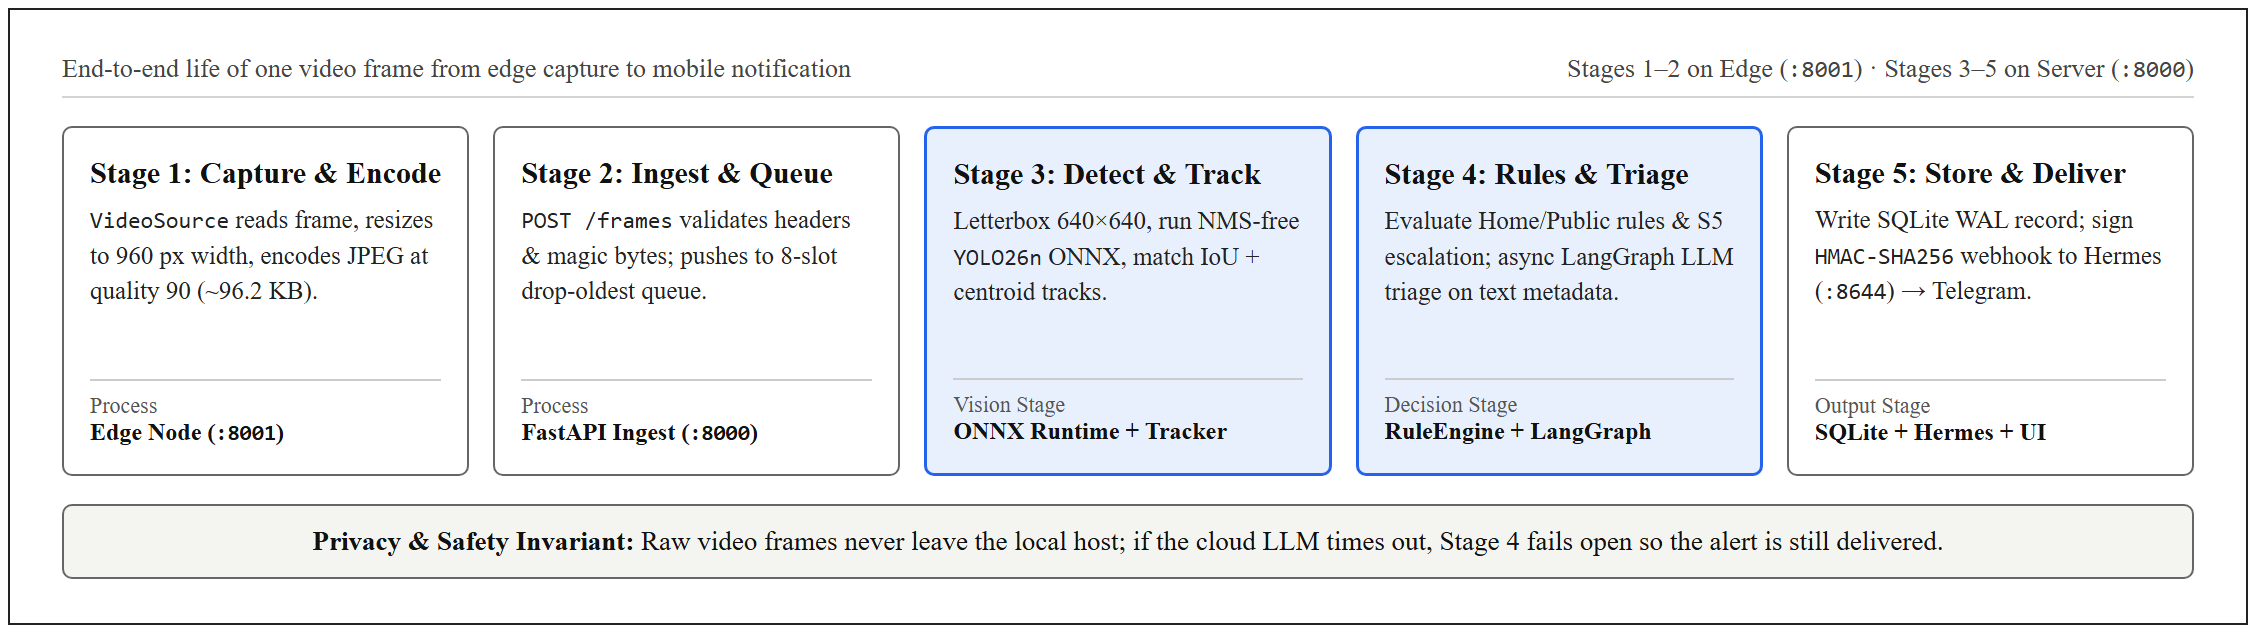
\includegraphics[width=0.98\linewidth]{figures/fig2_dataflow.png}
\caption{Ten-stage frame and event processing pipeline across the simulated IoT edge node (\code{:8001}), analysis server (\code{:8000}), asynchronous LangGraph triage worker, and Hermes webhook gateway (\code{:8644}).}
\label{fig:flow}
\end{figure}

\subsection{Timing and concurrency}

\begin{itemize}
  \item Rules use the edge capture timestamp, so queue delay does not distort dwell and loiter timers.
  \item The edge sends one frame at a time per device. The server queue is bounded (size 8) and drops the oldest frame when full, so stale frames are discarded in favour of fresh ones.
  \item A single lock serialises access to rule state and database writes from both ingestion paths (frames and injected events).
  \item The triage agent runs in a small thread pool so a slow LLM call never stalls the frame loop.
\end{itemize}

% ---------------- 4 ----------------
\section{The Simulated IoT Edge Node}

The edge node represents the camera-side IoT device. In a real deployment this would be a Raspberry Pi or similar board with a camera. Because that hardware was unavailable, the node is \textbf{simulated as its own server process} so that the architecture, the network boundary and the failure modes are still real.

\subsection{Why a separate process on its own port}

Running capture inside the analysis server would hide the boundary the project is about. A separate process on \code{:8001} means that the edge node can be started, paused, restarted or pointed at another server without touching the analysis side; that the only coupling is the frame upload; and that the same code can later be copied to a physical device. The server address is taken from the \code{AIIOT_SERVER_URL} variable (default \code{http://127.0.0.1:8000}).

\subsection{Edge control API}

\begin{table}[H]
\centering\small
\caption{Endpoints exposed by the edge node on port 8001}
\label{tab:ieee_7}
\begin{tabularx}{\textwidth}{|L{3.2cm}|L{1.6cm}|Y|}
\hline
\rowcolor{black!8} \textbf{Endpoint} & \textbf{Method} & \textbf{Purpose} \\ \hline
\code{/health} & GET & Role (\code{edge-node}), target server URL, streaming flag \\ \hline
\code{/edge/status} & GET & Active source, FPS, bandwidth, payload, frames sent, queue depth, source list \\ \hline
\code{/edge/config} & POST & Change source, device id, FPS, width, quality, streaming (validated) \\ \hline
\code{/edge/frame} & GET & Latest raw pre-inference JPEG for the preview box \\ \hline
\end{tabularx}
\end{table}

\subsection{Capture sources}

\code{VideoSource} accepts a webcam index, a local MP4 (looped at end of file), an RTSP or HTTP URL, or a YouTube URL resolved to a direct stream with \code{yt-dlp}. Live webcam capture sets the buffer size to one frame so processing never lags real time. Source strings are validated: a local file must be a direct child of \code{data/} ending in \code{.mp4}, which prevents path traversal.

\subsection{Encoder profile}

The default profile was raised during this project from 640 px width and JPEG quality 70 to 960 px and quality 90 so that small objects (bags, handbags) survive compression. Frame rate defaults to 5 FPS and can be changed live from the Edge Control Deck.

\begin{table}[H]
\centering\small
\caption{Default edge encoder profile}
\label{tab:ieee_8}
\begin{tabularx}{\textwidth}{|L{3.4cm}|L{2.2cm}|Y|}
\hline
\rowcolor{black!8} \textbf{Setting} & \textbf{Default} & \textbf{Reason} \\ \hline
Target FPS & 5 & Enough for dwell and loiter timers; low uplink \\ \hline
Frame width & 960 px & Keeps small bags detectable \\ \hline
JPEG quality & 90 & Reduces compression artefacts on small objects \\ \hline
Device id & \code{edge-01} & Tags every uploaded frame \\ \hline
Retry policy & back-off & Failed upload waits and retries; stale frames dropped \\ \hline
\end{tabularx}
\end{table}

\subsection{Video sources acquired for the demonstration}

Short stock clips do not simulate a continuous scene, so real security-camera footage was added. Table~\ref{tab:clips} lists every clip available in the source dropdown, with properties measured by OpenCV.

\begin{table}[H]
\centering\small
\caption{Video clips available to the simulated edge node}
\label{tab:clips}
\begin{tabularx}{\textwidth}{|L{3.8cm}|L{2.1cm}|L{1.4cm}|L{1.6cm}|Y|}
\hline
\rowcolor{black!8} \textbf{File} & \textbf{Resolution} & \textbf{FPS} & \textbf{Length} & \textbf{Sampled classes} \\ \hline
\code{demo.mp4} & 640$\times$480 & 15.0 & 46.0 s & bag scenario \\ \hline
\code{demo_attended.mp4} & 640$\times$480 & 15.0 & 36.0 s & bag with owner \\ \hline
\code{people-detection.mp4} & 768$\times$432 & 12.0 & 49.7 s & person \\ \hline
\code{person-bicycle-car.mp4} & 768$\times$432 & 12.0 & 53.9 s & person, bicycle, car \\ \hline
\code{worker-zone.mp4} & 1920$\times$1080 & 59.9 & 75.9 s & person \\ \hline
\code{store-aisle.mp4} & 720$\times$404 & 59.9 & 65.4 s & person \\ \hline
\code{car-detection.mp4} & 768$\times$432 & 12.5 & 30.2 s & car \\ \hline
\code{sec_cam_1.mp4} & 1920$\times$1080 & 12.5 & 48.4 s & car, person \\ \hline
\code{sec_cam_2.mp4} & 640$\times$360 & 30.0 & 130.6 s & cup, person \\ \hline
\code{sec_cam_3.mp4} & 640$\times$360 & 30.0 & 131.6 s & car, person \\ \hline
\code{sec_cam_4.mp4} & 640$\times$360 & 15.0 & 14.7 s & person \\ \hline
\end{tabularx}
\end{table}

The four \code{sec_cam} clips come from an open GitHub repository of security-camera footage; the others come from a public sample-video repository and from the project's own demos. Class names were found by running the detector on five sampled frames per clip, not over the whole clip.

\subsection{Playback timing caveat}

Clips recorded at 30 or 60 FPS are read one frame per emit tick, so at the 5 FPS target they play in slow motion relative to real time. Rule timers use wall-clock capture timestamps, not video time, so dwell and loiter durations in the live run are measured in real seconds of emission, not seconds of original footage. This is a known simplification of the simulation and is listed in Section~\ref{sec:limits}.

% ---------------- 5 ----------------
\section{Computer Vision and Tracking Pipeline}

\subsection{YOLO26n ONNX inference and letterbox geometry}

Detection runs through \code{ONNXRuntimeDetector} using a 9.8 MB \code{yolo26n.onnx} model on the CPU execution provider without requiring PyTorch at run time. Given an input BGR frame of height $H$ and width $W$, the aspect-preserving scale factor $r$ and symmetric grey padding $(\Delta w, \Delta h)$ for the $640\times 640$ network input are computed as:
\begin{equation}
r = \min\!\left(\frac{640}{H},\; \frac{640}{W}\right), \qquad
\Delta w = \frac{640 - \operatorname{round}(W \cdot r)}{2}, \qquad
\Delta h = \frac{640 - \operatorname{round}(H \cdot r)}{2}
\end{equation}
The model's NMS-free end-to-end head outputs a fixed tensor of shape $(1, 300, 6)$ where each row encodes $(x_1', y_1', x_2', y_2', c, k)$ in letterboxed pixel coordinates. For every row whose score $c$ exceeds the class-specific threshold $\tau_k$, coordinates are un-padded and normalised to $[0,1]$:
\begin{equation}
x_{1,2} = \operatorname{clip}\!\left(\frac{x_{1,2}' - \Delta w}{W \cdot r},\; 0,\; 1\right), \qquad
y_{1,2} = \operatorname{clip}\!\left(\frac{y_{1,2}' - \Delta h}{H \cdot r},\; 0,\; 1\right)
\end{equation}

\subsection{Accuracy improvements}

\begin{table}[H]
\centering\small
\caption{Accuracy measures added to the vision pipeline}
\label{tab:ieee_10}
\begin{tabularx}{\textwidth}{|L{3.6cm}|Y|L{3.3cm}|}
\hline
\rowcolor{black!8} \textbf{Measure} & \textbf{What it does} & \textbf{Where} \\ \hline
Higher uplink quality & 960 px and JPEG 90 keep small objects visible & \code{config.yaml} edge \\ \hline
Per-class thresholds & Person 0.40; backpack, handbag, suitcase 0.30; knife, scissors 0.35 & \code{detector.py} \\ \hline
Confidence hysteresis & Start a track at 0.40, keep it down to 0.30 & \code{tracker.py} \\ \hline
Multi-frame confirmation & \code{confirm_frames} counts hits before a track is active & \code{tracker.py} \\ \hline
Occlusion tolerance & A track survives up to 15 s of absence & \code{tracker.py} \\ \hline
Owner binding & Nearest person within radius 0.20 at spawn becomes owner & \code{tracker.py} \\ \hline
Stationary reset & A passer-by does not reset an unattended-bag timer unless stationary for 2 s & \code{tracker.py} \\ \hline
Class filtering & Optional allowed-class set per mode & \code{detector.py} \\ \hline
\end{tabularx}
\end{table}

\subsection{Tracker}

The tracker keeps per-class tracks for watched objects and a separate list of person tracks. Detections are matched greedily by overlap (IoU), then by centroid distance within 0.25 of the frame. Each track stores first and last seen times, a short history, an anchor box about five seconds old, the last time a person was near it, the bound owner, the last person near it and a hit counter. Person tracks also expose a speed estimate (normalised centre movement per second), used by the running rule.

\subsection{Offline evaluation harness}

\code{scripts/eval.py} replays video clips through the same detector and rule engine and compares which rules fired with a small label file. It was written so that accuracy changes could be measured instead of guessed.

\begin{table}[H]
\centering\small
\caption{Result of the offline evaluation on the two labelled clips}
\label{tab:ieee_11}
\begin{tabularx}{\textwidth}{|L{3.4cm}|Y|Y|L{1.9cm}|}
\hline
\rowcolor{black!8} \textbf{Clip} & \textbf{Rules that fired} & \textbf{Expected} & \textbf{Outcome} \\ \hline
\code{demo.mp4} & \code{object_dwell}, \code{occupancy_spike}, \code{rapid_gathering}, \code{unexpected_object} & \code{object_dwell}, \code{unexpected_object} & 2 TP \\ \hline
\code{demo_attended.mp4} & \code{unexpected_object} & \code{unexpected_object}; \code{object_dwell} forbidden & 1 TP, 0 FP \\ \hline
\textbf{Total} & & & \textbf{P = 1.00, R = 1.00} \\ \hline
\end{tabularx}
\end{table}

\textbf{Honest reading.} The first run scored recall 0.67 because the label for \code{demo_attended.mp4} expected an occupancy spike that the clip does not produce; the label was then corrected to match the observed behaviour. The 1.00/1.00 figure therefore comes from a tiny, self-labelled set and demonstrates that the harness works, not that accuracy is generally perfect. Extra rules that fired but were not forbidden (\code{occupancy_spike}, \code{rapid_gathering}) are not counted as false positives by this simple scoring. A larger independently labelled set is future work.

% ---------------- 6 ----------------
\section{Dual-Mode Rule Engine}

A single \code{RuleEngine} switches between \textbf{Home Security} and \textbf{Public Space} through the \code{mode} setting, changed at run time with \code{POST /mode}. Spatial rules use OpenCV polygon tests on the bottom centre of a person's box, tripwire rules use the sign of a cross product against a configured line, and time rules use the local clock.

\subsection{Arming states (Home mode)}

\begin{table}[H]
\centering\small
\caption{Home arming states and the rules each activates}
\label{tab:ieee_12}
\begin{tabularx}{\textwidth}{|L{3.0cm}|Y|}
\hline
\rowcolor{black!8} \textbf{Arming state} & \textbf{Active behaviour} \\ \hline
\code{disarmed} & Camera-health rules only (offline, blocked, moved) \\ \hline
\code{armed_home} & Exterior zones; interior zones are skipped; person-down and vehicle rules \\ \hline
\code{armed_night} & All zones including interior; night-person rule; entry loitering raised to critical \\ \hline
\code{armed_away} & Full suite including interior intrusion, parcel and valuable-removal rules \\ \hline
\end{tabularx}
\end{table}

\subsection{Configured zones and geometric formulations}

Spatial rules evaluate each tracked person's bottom-centre anchor point (foot point) against normalised polygon vertices in $[0,1]^2$ using OpenCV's point-in-polygon test, while directional tripwires evaluate the signed cross product between successive track centroids and the configured line segment $\mathbf{a}\to\mathbf{b}$:
\begin{equation}
\mathbf{p}_{\text{foot}} = \left(\frac{x_1 + x_2}{2},\; y_2\right), \qquad
s(\mathbf{p}) = (b_x - a_x)(p_y - a_y) - (b_y - a_y)(p_x - a_x)
\end{equation}
A tripwire crossing is registered when $\operatorname{sign}(s(\mathbf{p}_{t-1})) \neq \operatorname{sign}(s(\mathbf{p}_t))$ and the displacement vector aligns with the configured forbidden direction. Fig.~\ref{fig:zones} illustrates the normalised spatial zones and tripwire geometry for both operating modes, and the zone parameters are listed in the tables below.

\begin{figure}[H]
\centering
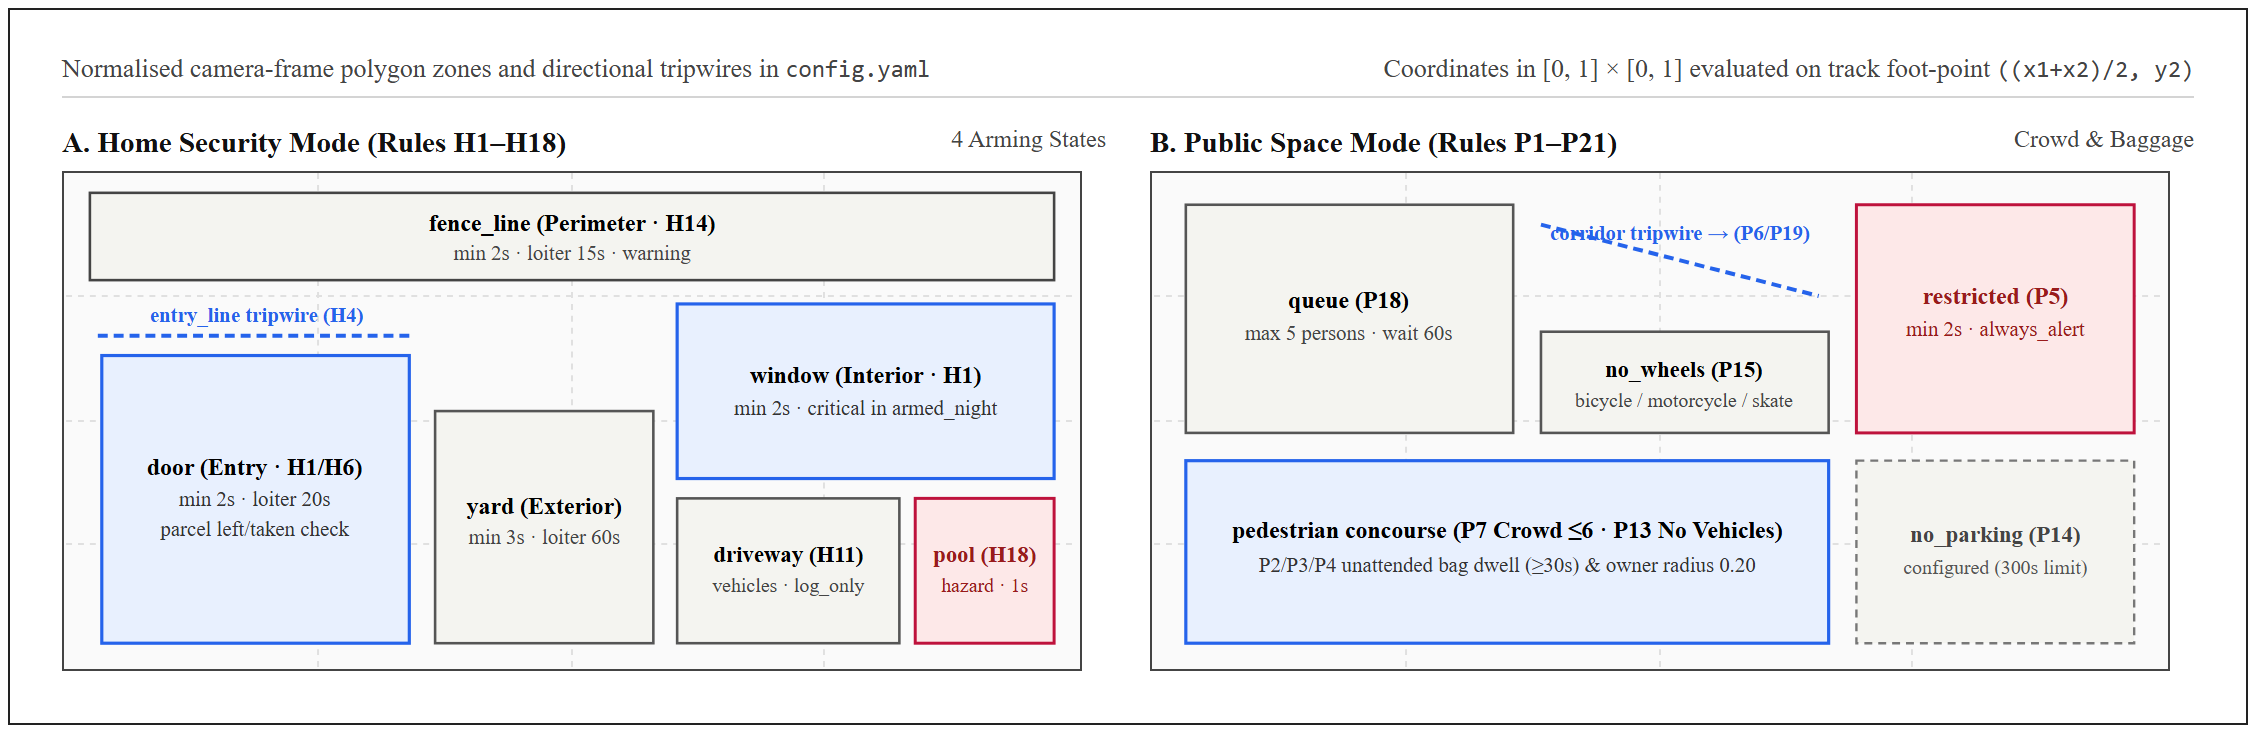
\includegraphics[width=0.98\linewidth]{figures/fig4_zones.png}
\caption{Normalised spatial polygon zones and tripwire geometry configured in \code{config.yaml} for Home Security mode (\code{H1}--\code{H18}) and Public Space mode (\code{P1}--\code{P21}).}
\label{fig:zones}
\end{figure}

\begin{table}[H]
\centering\small
\caption{Home zones in \code{config.yaml} (normalised polygons)}
\label{tab:ieee_13}
\begin{tabularx}{\textwidth}{|L{2.4cm}|L{2.2cm}|L{1.4cm}|L{1.6cm}|L{1.8cm}|Y|}
\hline
\rowcolor{black!8} \textbf{Zone} & \textbf{Kind} & \textbf{Min s} & \textbf{Loiter s} & \textbf{Severity} & \textbf{Purpose} \\ \hline
\code{door} & entry & 2 & 20 & warning & Front entrance \\ \hline
\code{window} & interior & 2 & 15 & critical & Interior window area \\ \hline
\code{yard} & exterior & 3 & 60 & warning & Garden or front yard \\ \hline
\code{driveway} & driveway & 2 & 600 & info & Vehicles \\ \hline
\code{fence_line} & perimeter & 2 & 15 & warning & Boundary approach \\ \hline
\code{pool} & hazard & 1 & 10 & critical & Child safety \\ \hline
\end{tabularx}
\end{table}

\begin{table}[H]
\centering\small
\caption{Public-space zones and lines in \code{config.yaml}}
\label{tab:ieee_14}
\begin{tabularx}{\textwidth}{|L{2.6cm}|L{2.2cm}|Y|}
\hline
\rowcolor{black!8} \textbf{Zone / line} & \textbf{Kind} & \textbf{Parameter} \\ \hline
\code{restricted} & restricted & Minimum 2 s inside; critical \\ \hline
\code{pedestrian} & pedestrian & Crowd limit 6; vehicles raise an alert \\ \hline
\code{no_parking} & no\_parking & Still limit 300 s (rule not implemented, Section~\ref{sec:limits}) \\ \hline
\code{no_wheels} & no\_wheels & Bicycles, skateboards, motorcycles \\ \hline
\code{queue} & queue & Limit 5 persons, wait 60 s \\ \hline
\code{corridor} & line & Allowed direction left to right \\ \hline
\end{tabularx}
\end{table}

\subsection{Shared camera-health rules}

\begin{table}[H]
\centering\small
\caption{Shared rules (both modes)}
\label{tab:ieee_15}
\begin{tabularx}{\textwidth}{|L{1.0cm}|L{3.7cm}|Y|L{1.9cm}|}
\hline
\rowcolor{black!8} \textbf{ID} & \textbf{Rule} & \textbf{Trigger and defaults} & \textbf{Policy} \\ \hline
S1 & \code{camera_offline} & No frame for 30 s & \cellcolor{red!12}always alert \\ \hline
S2 & \code{camera_tamper_blocked} & Mean luminance below 15 or Laplacian variance below 20 for 5 s & \cellcolor{red!12}always alert \\ \hline
S3 & \code{camera_tamper_moved} & Histogram difference above 0.65 sustained 5 s against a slowly updated reference & \cellcolor{blue!10}review \\ \hline
S4 & low-visibility mode & Raise thresholds at night & \cellcolor{red!12}\textbf{not implemented} \\ \hline
S5 & repeat escalation & Same rule 3 times in 10 minutes raises severity one level & modifier \\ \hline
S6 & arming state & Selects active Home rules & \cellcolor{green!15}implemented \\ \hline
S7 & quiet-hours digest & Summarise non-critical events & \cellcolor{red!12}\textbf{not implemented} \\ \hline
\end{tabularx}
\end{table}

\subsection{Home Security rules}

\begin{table}[H]
\centering\footnotesize
\caption{Home Security rules implemented in \code{rules.py} (part 1)}
\label{tab:ieee_16}
\begin{tabularx}{\textwidth}{|L{0.8cm}|L{4.5cm}|Y|L{1.7cm}|}
\hline
\rowcolor{black!8} \textbf{ID} & \textbf{Rule} & \textbf{Trigger and defaults} & \textbf{Policy} \\ \hline
H1 & \code{person_in_zone} & Person's foot point inside a zone polygon for the zone's minimum seconds & \cellcolor{blue!10}review \\ \hline
H2 & \code{night_person} & Any person during the night window (22:00--06:00) or while armed at night & \cellcolor{blue!10}review \\ \hline
H3 & \code{loitering} & Person stationary in a zone beyond its loiter seconds & \cellcolor{blue!10}review \\ \hline
H4 & \code{zone_entry_exit} & Person track crosses a configured tripwire line & \cellcolor{black!6}log only \\ \hline
H5 & \code{multiple_persons_entry} & Two or more persons in an entry zone at once & \cellcolor{blue!10}review \\ \hline
H6 & \code{object_left_at_door} & Bag-class object still in the door zone for 10 s without a person near & \cellcolor{blue!10}review \\ \hline
H7 & \code{object_taken_from_door} & Door-zone object disappears after 3 s while a person was near & \cellcolor{blue!10}review \\ \hline
H8 & \code{valuable_removed} & Laptop or television present 5 minutes then missing near a person & \cellcolor{red!12}always alert \\ \hline
H9 & \code{person_down} & Person box width/height $\ge 1.2$, stationary 10 s & \cellcolor{red!12}always alert \\ \hline
\end{tabularx}
\end{table}

\begin{table}[H]
\centering\footnotesize
\caption{Home Security rules implemented in \code{rules.py} (part 2)}
\label{tab:ieee_17}
\begin{tabularx}{\textwidth}{|L{0.8cm}|L{4.5cm}|Y|L{1.7cm}|}
\hline
\rowcolor{black!8} \textbf{ID} & \textbf{Rule} & \textbf{Trigger and defaults} & \textbf{Policy} \\ \hline
H10 & \code{prolonged_inactivity} & Person stationary for 30 minutes & \cellcolor{blue!10}review \\ \hline
H11 & \code{vehicle_in_driveway} & Car, motorcycle or truck in the driveway zone & \cellcolor{black!6}log only \\ \hline
H12 & \code{vehicle_lingering} & Vehicle in driveway for 10 minutes & \cellcolor{blue!10}review \\ \hline
H13 & \code{sharp_object_near_person} & Knife or scissors within 0.15 of a person & \cellcolor{blue!10}review \\ \hline
H14 & \code{fence_or_wall_approach} & Person in the perimeter zone for its minimum seconds & \cellcolor{blue!10}review \\ \hline
H15 & \code{repeat_visit_casing} & Three or more distinct person tracks in a zone within 30 minutes & \cellcolor{blue!10}review \\ \hline
H16 & pet filtering & Dogs and cats ignored for person rules & \cellcolor{green!15}implemented \\ \hline
H17 & \code{pet_alone_in_restricted_zone} & Pet in hazard or perimeter zone with no person visible & \cellcolor{black!6}log only \\ \hline
H18 & \code{child_near_hazard_zone} & Person box shorter than 0.25 of the frame in a hazard zone & \cellcolor{red!12}always alert \\ \hline
\end{tabularx}
\end{table}

\subsection{Public Space rules}

\begin{table}[H]
\centering\footnotesize
\caption{Public Space rules implemented in \code{rules.py} (part 1)}
\label{tab:ieee_18}
\begin{tabularx}{\textwidth}{|L{0.8cm}|L{4.5cm}|Y|L{1.7cm}|}
\hline
\rowcolor{black!8} \textbf{ID} & \textbf{Rule} & \textbf{Trigger and defaults} & \textbf{Policy} \\ \hline
P1 & \code{occupancy_spike} & More than 3 persons in frame & \cellcolor{blue!10}review \\ \hline
P2 & \code{unexpected_object} & Watched bag present 5 s & \cellcolor{blue!10}review \\ \hline
P3 & \code{object_dwell} & No person near a watched bag for 30 s & \cellcolor{blue!10}review \\ \hline
P4 & \code{abandoned_after_owner_left} & Bound owner absent 20 s & \cellcolor{blue!10}review \\ \hline
P5 & \code{restricted_area_intrusion} & Person inside restricted polygon 2 s & \cellcolor{red!12}always alert \\ \hline
P6 & \code{wrong_way_or_tripwire} & Crossing a line against the allowed direction & \cellcolor{blue!10}review \\ \hline
P7 & \code{zone_crowd_density} & More persons in a zone than its limit & \cellcolor{blue!10}review \\ \hline
P8 & \code{rapid_gathering} & Count rises 100\% in 10 s to at least 4 & \cellcolor{blue!10}review \\ \hline
P9 & \code{sudden_dispersal} & Count falls 60\% in 5 s from at least 5 & \cellcolor{red!12}always alert \\ \hline
P10 & \code{loitering} & Person stationary 120 s & \cellcolor{blue!10}review \\ \hline
\end{tabularx}
\end{table}

\begin{table}[H]
\centering\footnotesize
\caption{Public Space rules implemented in \code{rules.py} (part 2)}
\label{tab:ieee_19}
\begin{tabularx}{\textwidth}{|L{0.8cm}|L{5.8cm}|Y|L{1.7cm}|}
\hline
\rowcolor{black!8} \textbf{ID} & \textbf{Rule} & \textbf{Trigger and defaults} & \textbf{Policy} \\ \hline
P11 & \code{person_down} & Aspect ratio $\ge 1.2$, stationary 10 s & \cellcolor{red!12}always alert \\ \hline
P12 & \code{running_or_fast_movement} & Person speed at least 0.35 frame-widths per second & \cellcolor{blue!10}review \\ \hline
P13 & \code{vehicle_in_pedestrian_zone} & Vehicle inside pedestrian polygon & \cellcolor{red!12}always alert \\ \hline
P14 & illegal parking & Vehicle still in no-parking zone & \cellcolor{red!12}\textbf{not implemented} \\ \hline
P15 & \code{bicycle_or_scooter_in_restricted_zone} & Bicycle, skateboard or motorcycle in no-wheels zone & \cellcolor{blue!10}review \\ \hline
P16 & \code{multiple_unattended_objects} & Two or more unattended bags & \cellcolor{blue!10}review \\ \hline
P17 & \code{bag_taken_by_other_person} & Non-owner interacts with an owned bag & \cellcolor{blue!10}review \\ \hline
P18 & \code{queue_or_wait_overflow} & Queue over its limit for 60 s & \cellcolor{blue!10}review \\ \hline
P19 & \code{capacity_exceeded} & Net count through the line above 20 & \cellcolor{blue!10}review \\ \hline
P20 & \code{after_hours_presence} & Person outside 08:00--22:00 & \cellcolor{blue!10}review \\ \hline
P21 & \code{sharp_object_near_person} & Knife or scissors near a person & \cellcolor{blue!10}review \\ \hline
\end{tabularx}
\end{table}

\subsection{Cooldowns, escalation and policies}

Each rule fires at most once per cooldown (10 s by default) per rule, track and zone. When the same rule has fired three times within ten minutes its severity is raised one level, which explains why the same event type appears as \textbf{warning} and then \textbf{critical} in the live Telegram alerts (Section~\ref{sec:results}). Rules are tagged with one of three policies that tell the triage agent how much freedom it has: \code{review} (the LLM may suppress), \code{always_alert} (the LLM may only add a reason) and \code{log_only} (stored, never pushed).

\subsection{Rule tiers and limits}

\begin{table}[H]
\centering\small
\caption{What the COCO-80 detector can and cannot support}
\label{tab:ieee_20}
\begin{tabularx}{\textwidth}{|L{2.0cm}|Y|Y|}
\hline
\rowcolor{black!8} \textbf{Tier} & \textbf{Meaning} & \textbf{Examples} \\ \hline
A & Works with the current detector, tracker, geometry and time & Zone intrusion, night person, crowd count, dwell \\ \hline
B & Needs person--object tracking beyond simple IoU & Owner hand-over, bag taken, capacity counting (implemented approximately) \\ \hline
C & Needs another model & Faces, fire and smoke, weapons beyond knife, fighting, fall pose, licence plates, parcels \\ \hline
\end{tabularx}
\end{table}

% ---------------- 7 ----------------
\section{Agentic Triage with LangGraph}

\subsection{Why an agent at all}

Rules are precise but context-free. The same \code{person_in_zone} event means something different at 02:10 while armed for the night than at noon while the family is home. A language model can weigh that context, repeats and recent history in plain language, and can write a one-line reason that the owner can read. The design goal is to let the model \emph{filter and explain} without being able to \emph{hide} safety-critical events.

\subsection{Workflow}

Fig.~\ref{fig:langgraph} depicts the four-node LangGraph state machine that processes every rule trigger.

\begin{figure}[H]
\centering
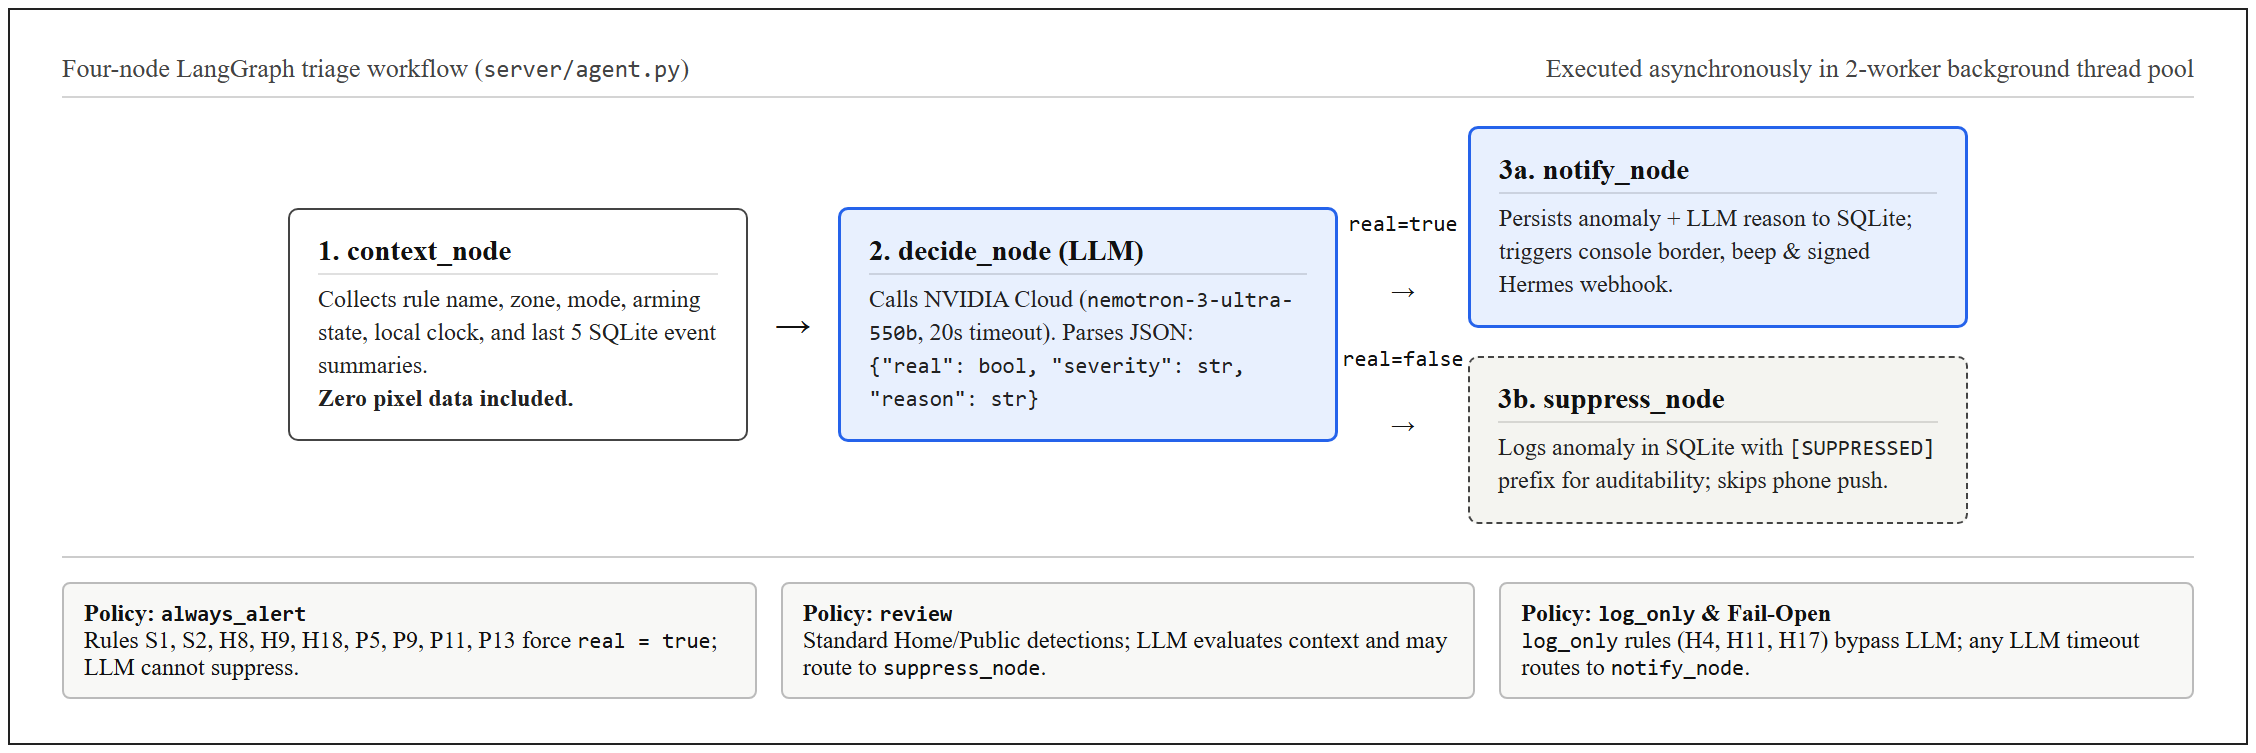
\includegraphics[width=0.98\linewidth]{figures/fig3_langgraph.png}
\caption{The four-node LangGraph triage workflow. Rules tagged \code{always_alert} cannot be routed to \code{suppress}; any network error routes to \code{notify}.}
\label{fig:langgraph}
\end{figure}

\subsection{What the model sees}

The prompt contains the rule name, policy, zone, initial severity and detail text, the deployment mode and arming state, the local time, and a short summary of the five most recent detection events from the database (class, count, average confidence). It contains no image, no pixel data and no file path. The model is asked to reply with a single JSON object with the keys \code{real}, \code{severity} and \code{reason}; the reply is parsed defensively by extracting the first JSON object in the text.

\begin{table}[H]
\centering\small
\caption{Privacy boundary of the agent}
\label{tab:ieee_21}
\begin{tabularx}{\textwidth}{|L{4.0cm}|L{2.2cm}|Y|}
\hline
\rowcolor{black!8} \textbf{Data item} & \textbf{Sent to LLM} & \textbf{Note} \\ \hline
Video frames and JPEGs & \No & Never leave the local machine \\ \hline
Bounding boxes and pixels & \No & Used locally only \\ \hline
Rule name, zone, mode, arming & \Yes & Short text \\ \hline
Local time of the event & \Yes & Needed for night reasoning \\ \hline
Last five event summaries & \Yes & Class names, counts, confidence \\ \hline
Device id & \Yes & Camera label \\ \hline
\end{tabularx}
\end{table}

\subsection{Safety properties}

\begin{itemize}
  \item \textbf{Fail-open.} Any exception (timeout, HTTP error, malformed JSON) produces an alert with the reason text \code{fail-open (...)}. The agent can never hide an alert because of an outage.
  \item \textbf{Always-alert rules.} For rules in the always-alert set (camera offline or blocked, person down, valuable removed, restricted-area intrusion, sudden dispersal, vehicle in pedestrian zone, child near hazard) the model's \code{real} flag is overridden to true.
  \item \textbf{Log-only rules.} These bypass the model and are stored with a \code{[SUPPRESSED]} marker; the live console shows one such record for a vehicle in the driveway.
  \item \textbf{Non-blocking.} A two-worker thread pool runs the graph so the frame loop never waits for the model.
\end{itemize}

\subsection{Model choice history}

The first plan used Ollama cloud models. Testing showed that every cloud model on the account returned HTTP 402 (credits or subscription required) and that one had been retired, so Ollama was dropped. The agent now calls an OpenAI-compatible endpoint on NVIDIA's cloud with the model \code{nvidia/nemotron-3-ultra-550b-a55b}. A probe returned valid JSON in 4.5 s; three alternative models timed out at 40 s in the same probe. The model name, base URL and timeout are configuration, and the API key is read from a git-ignored \code{.env} file.

\begin{table}[H]
\centering\small
\caption{Model probe results before settling on the agent model}
\label{tab:ieee_22}
\begin{tabularx}{\textwidth}{|L{4.6cm}|L{2.6cm}|Y|}
\hline
\rowcolor{black!8} \textbf{Model (endpoint)} & \textbf{Result} & \textbf{Note} \\ \hline
Ollama cloud models (several) & HTTP 402 & Account had no credits \\ \hline
One Ollama model & retired & Replaced by vendor suggestion \\ \hline
\code{nemotron-3-ultra-550b-a55b} (NVIDIA) & valid JSON, 4.5 s & Chosen \\ \hline
Three other NVIDIA models & timed out at 40 s & Not used \\ \hline
\end{tabularx}
\end{table}

% ---------------- 8 ----------------
\section{Alert Delivery with Hermes Agent and Telegram}

\subsection{Roles}

LangGraph decides \emph{whether} to alert. Hermes Agent only \emph{delivers}. This separation keeps the decision logic inside the project and keeps the messaging credentials (Telegram bot token) inside the Hermes gateway.

\subsection{Webhook}

When the triage graph notifies, \code{alerts.fire()} lights the on-screen alert border for 15 seconds, prints a console banner, beeps and calls \code{send_hermes_webhook()}. That function builds a small JSON payload, signs the exact bytes with HMAC-SHA256 using a secret from the environment, and posts it to \code{http://127.0.0.1:8644/webhooks/house-alert} with an \code{X-Hub-Signature-256} header. If the secret is missing the call is skipped rather than sending an unsigned request. A short timeout and exception handling mean a gateway outage is logged, never raised. The Hermes route was created in direct-delivery mode, so no extra LLM call or cost is incurred by the messaging step.

Every outbound webhook payload $M$ is signed over its exact UTF-8 byte representation using the shared secret $K$ (\code{HERMES\_WEBHOOK\_SECRET}):
\begin{equation}
\text{X-Hub-Signature-256} = \texttt{"sha256="} \;\Vert\; \operatorname{hex}\!\left(\operatorname{HMAC-SHA256}(K,\, M)\right)
\end{equation}
Fig.~\ref{fig:webhookseq} illustrates the four-stage cryptographic signing and delivery sequence from \code{notify\_node} to the Telegram mobile client.

\begin{figure}[H]
\centering
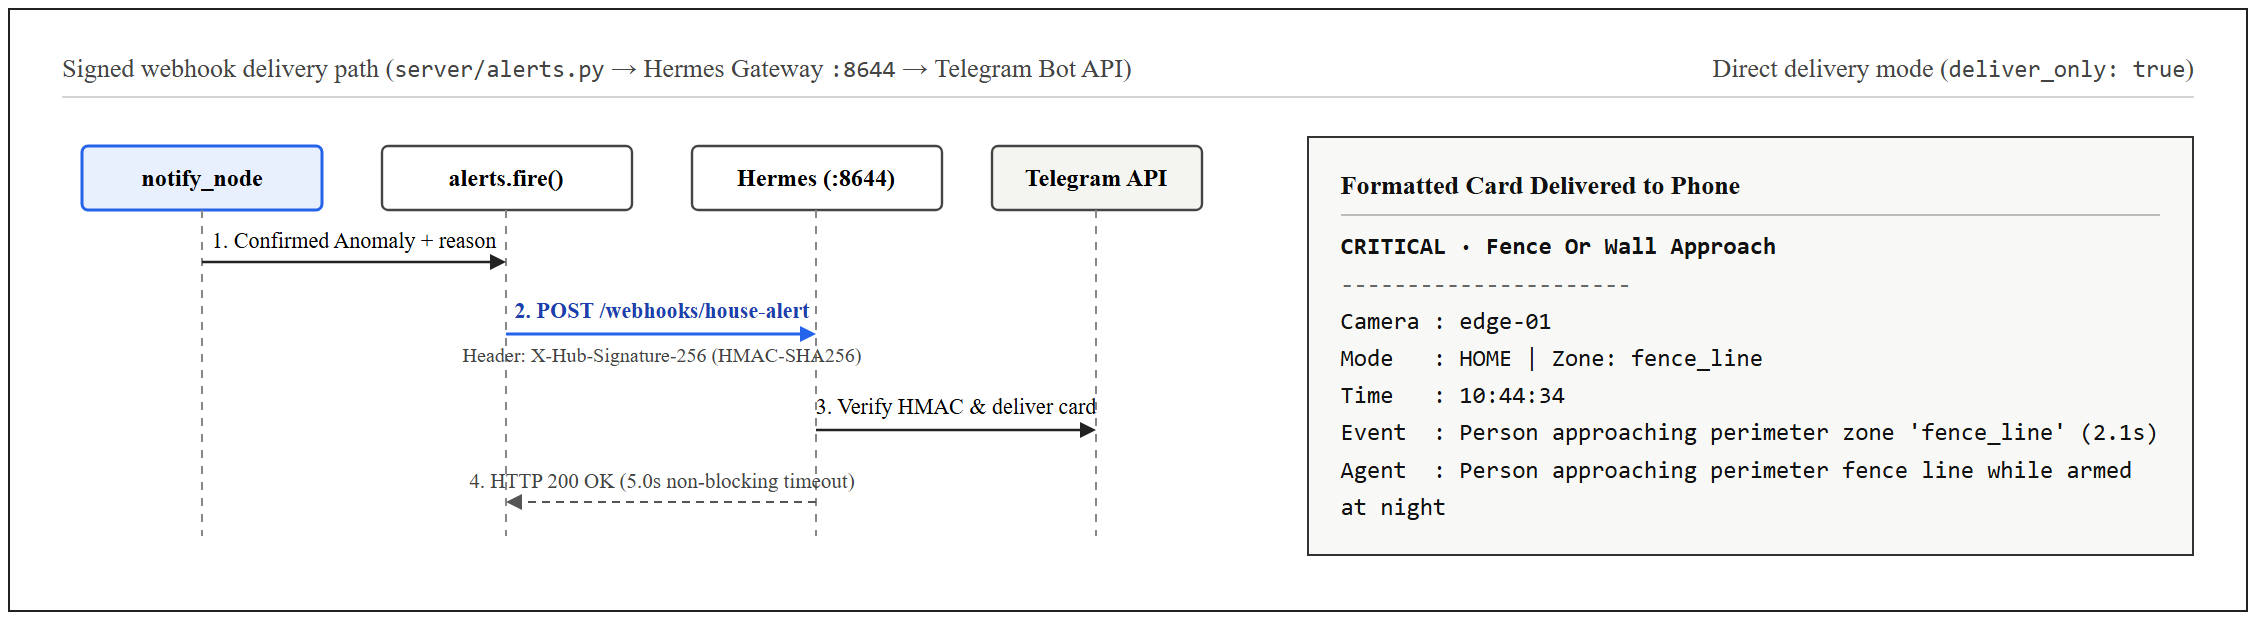
\includegraphics[width=0.98\linewidth]{figures/fig8_webhook_seq.png}
\caption{Signed webhook and Telegram mobile alert delivery pipeline (\code{server/alerts.py} $\rightarrow$ Hermes Agent \code{:8644} $\rightarrow$ Telegram Bot API).}
\label{fig:webhookseq}
\end{figure}

\subsection{Message format}

The first version of the alert was a single line. It was replaced by a structured card that reads well on a phone: a severity icon and title, a divider, then camera, mode and zone, time, the event text and the agent's reason.

\begin{table}[H]
\centering\small
\caption{Fields of the Telegram alert card}
\label{tab:ieee_23}
\begin{tabularx}{\textwidth}{|L{3.0cm}|L{3.2cm}|Y|}
\hline
\rowcolor{black!8} \textbf{Line} & \textbf{Source} & \textbf{Example from the live run} \\ \hline
Severity and title & Rule severity and name & Warning, Fence Or Wall Approach \\ \hline
Camera & Device id & \code{edge-01} \\ \hline
Mode and zone & Mode, zone of the event & HOME, \code{fence_line} \\ \hline
Time & Event timestamp & 10:44:31 \\ \hline
Event & Rule detail text & Person approaching perimeter zone (2.1 s) \\ \hline
Agent & LLM reason or fail-open note & Person detected approaching fence line during armed night mode \\ \hline
\end{tabularx}
\end{table}

\subsection{Gateway operation}

The Hermes gateway runs as its own process (\code{hermes gateway run}) on port 8644. On Windows a gateway started from a tool shell can be killed when that shell exits, so it is started in a normal command window for the demonstration. The webhook listener accepts connections on all interfaces by default; requests are signed, but binding it to the loopback address would be a sensible hardening step before real use.

% ---------------- 9 ----------------
\section{Web Consoles}

Two Vite and React consoles share one design system and are served on separate ports. Each talks only to the backend that owns the function it controls.

\begin{table}[H]
\centering\small
\caption{The two web consoles}
\label{tab:ieee_24}
\begin{tabularx}{\textwidth}{|L{3.2cm}|L{1.4cm}|L{3.0cm}|Y|}
\hline
\rowcolor{black!8} \textbf{Console} & \textbf{Port} & \textbf{Talks to} & \textbf{Main features} \\ \hline
Analytics Console & 5173 & Server \code{:8000} & Annotated YOLO feed, KPI strip, person-count timeline, anomaly vault, detection ledger, node list \\ \hline
Edge Control Deck & 5174 & Edge \code{:8001} and server \code{:8000} & Video source dropdown with an \emph{Other} URL field, mode and arming switch, clip rule hints, encoder sliders, synthetic rule injector \\ \hline
\end{tabularx}
\end{table}

\subsection{Edge Control Deck}

The source selector is a drop-down of every clip plus the webcam; choosing \emph{Other} reveals a text field for a custom path, RTSP or YouTube URL. The mode panel switches between Home and Public and, in Home, between the four arming states. For the active clip the panel prints the rules that clip is expected to exercise and offers a one-click button to apply the recommended mode. The injector tab provides one-click synthetic triggers (R1--R3, P5, P13, H1, H6, H9, H11) that post scripted detections to the server, which was used during development when a clip had not yet crossed a dwell threshold.

\subsection{Analytics Console}

The console polls statistics, anomalies, events, devices and health every 650 ms and the annotated frame every 260 ms. A red notice bar shows the latest active alert; tabs list anomalies, detections and nodes. Fig.~\ref{fig:analytics} is a capture from the live run.

\begin{figure}[H]
\centering
\fbox{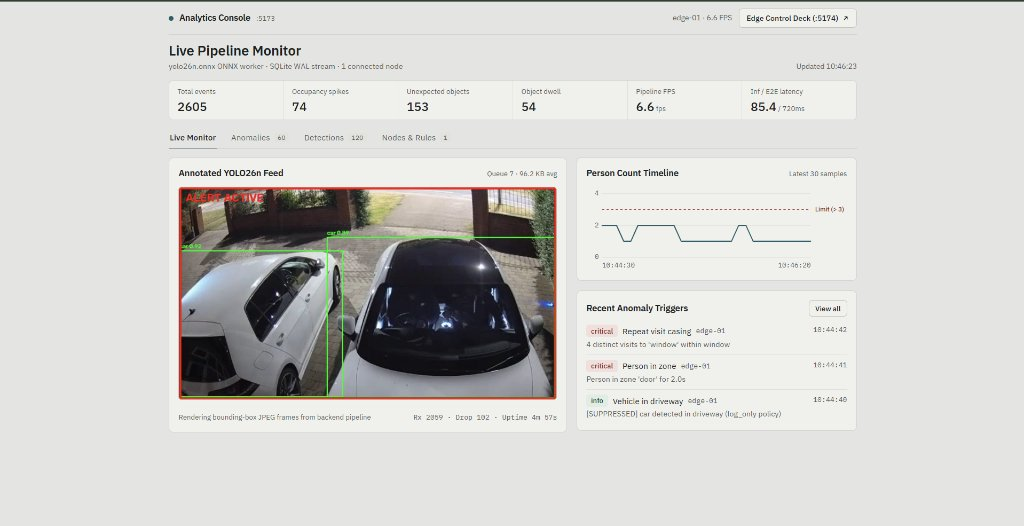
\includegraphics[width=0.96\linewidth]{figures/analytics_live.jpg}}
\caption{Analytics Console during the live run (17 November 2026, 10:46): annotated feed with the red \emph{Alert Active} border, KPI strip, person-count timeline and recent anomaly triggers, including a \code{[SUPPRESSED]} log-only vehicle record.}
\label{fig:analytics}
\end{figure}

% ---------------- 10 ----------------
\section{Security Hardening and Privacy Model}

\begin{table}[H]
\centering\small
\caption{Security and privacy controls}
\label{tab:ieee_25}
\begin{tabularx}{\textwidth}{|L{4.0cm}|Y|L{2.6cm}|}
\hline
\rowcolor{black!8} \textbf{Control} & \textbf{Implementation} & \textbf{Verified by} \\ \hline
API key & Optional \code{AIIOT_API_KEY}; mandatory when bound to all interfaces; missing key gives 401, wrong key gives 403 & Tests \\ \hline
Payload size limit & \code{Content-Length} above 2 MB rejected with 413 before the body is read & Tests \\ \hline
Image dimension limit & JPEG header larger than 4096$\times$4096 rejected with 400 & Tests \\ \hline
JPEG magic check & Non-JPEG bodies rejected with 400 & Tests \\ \hline
Source validation & Camera index, allowed URL schemes, or direct child \code{data/*.mp4}; traversal rejected & Tests \\ \hline
CORS allow-list & Only \code{localhost:5173} and \code{localhost:5174} & Test \\ \hline
Webhook signing & HMAC-SHA256 header with secret from environment & Test \\ \hline
Secrets handling & API keys and webhook secret in a git-ignored \code{.env} & Inspection \\ \hline
No images to the cloud & Agent receives text metadata only & Design and code \\ \hline
\end{tabularx}
\end{table}

\subsection{Residual risks}

\begin{itemize}
  \item The Hermes webhook listener binds all interfaces by default; the HMAC protects it, but loopback binding is safer.
  \item The Telegram bot token appeared in a shared screenshot during development and should be revoked and reissued before any real deployment.
  \item Alert text goes through Telegram's servers; it contains camera name, zone and time but no image.
  \item The edge control API (\code{:8001}) has no authentication when run locally; the API-key check applies when it is exposed beyond loopback.
\end{itemize}

% ---------------- 11 ----------------
\section{Experimental Setup and Results}\label{sec:results}

\subsection{Setup}

All measurements were taken on one laptop with an Intel Core i5-12500H CPU. For the live run the following were running at the same time: the analysis server (\code{:8000}), the simulated IoT edge node (\code{:8001}), the Analytics and Edge consoles (\code{:5173}, \code{:5174}) in a browser, the Hermes gateway (\code{:8644}), and calls out to the cloud LLM. The edge node streamed a security-camera clip of a driveway; the system was in \code{home} mode, \code{armed_night}.

\subsection{Isolated pipeline benchmark}

Table~\ref{tab:bench} and Fig.~\ref{fig:payload} summarise the uplink payload and latency measurements across ingestion modes.

\begin{table}[H]
\centering\small
\caption{Measured pipeline performance, 640$\times$480 at 5 FPS}
\label{tab:bench}
\begin{tabularx}{\textwidth}{|L{4.0cm}|L{1.9cm}|L{2.3cm}|L{2.0cm}|Y|}
\hline
\rowcolor{black!8} \textbf{Mode} & \textbf{Payload} & \textbf{Bandwidth} & \textbf{Inference} & \textbf{End to end} \\ \hline
Raw BGR (baseline) & 900.0 KB & 4,500 KB/s & -- & -- \\ \hline
Edge JPEG, quality 70 & 23.3--31.0 KB & 116.5--155.0 KB/s & 27.6 ms (about 36 FPS) & 50.5--67.0 ms \\ \hline
Event JSON (\code{/events}) & about 0.18 KB & about 0.9 KB/s & -- & under 5 ms \\ \hline
\end{tabularx}
\end{table}

\begin{figure}[H]
\centering
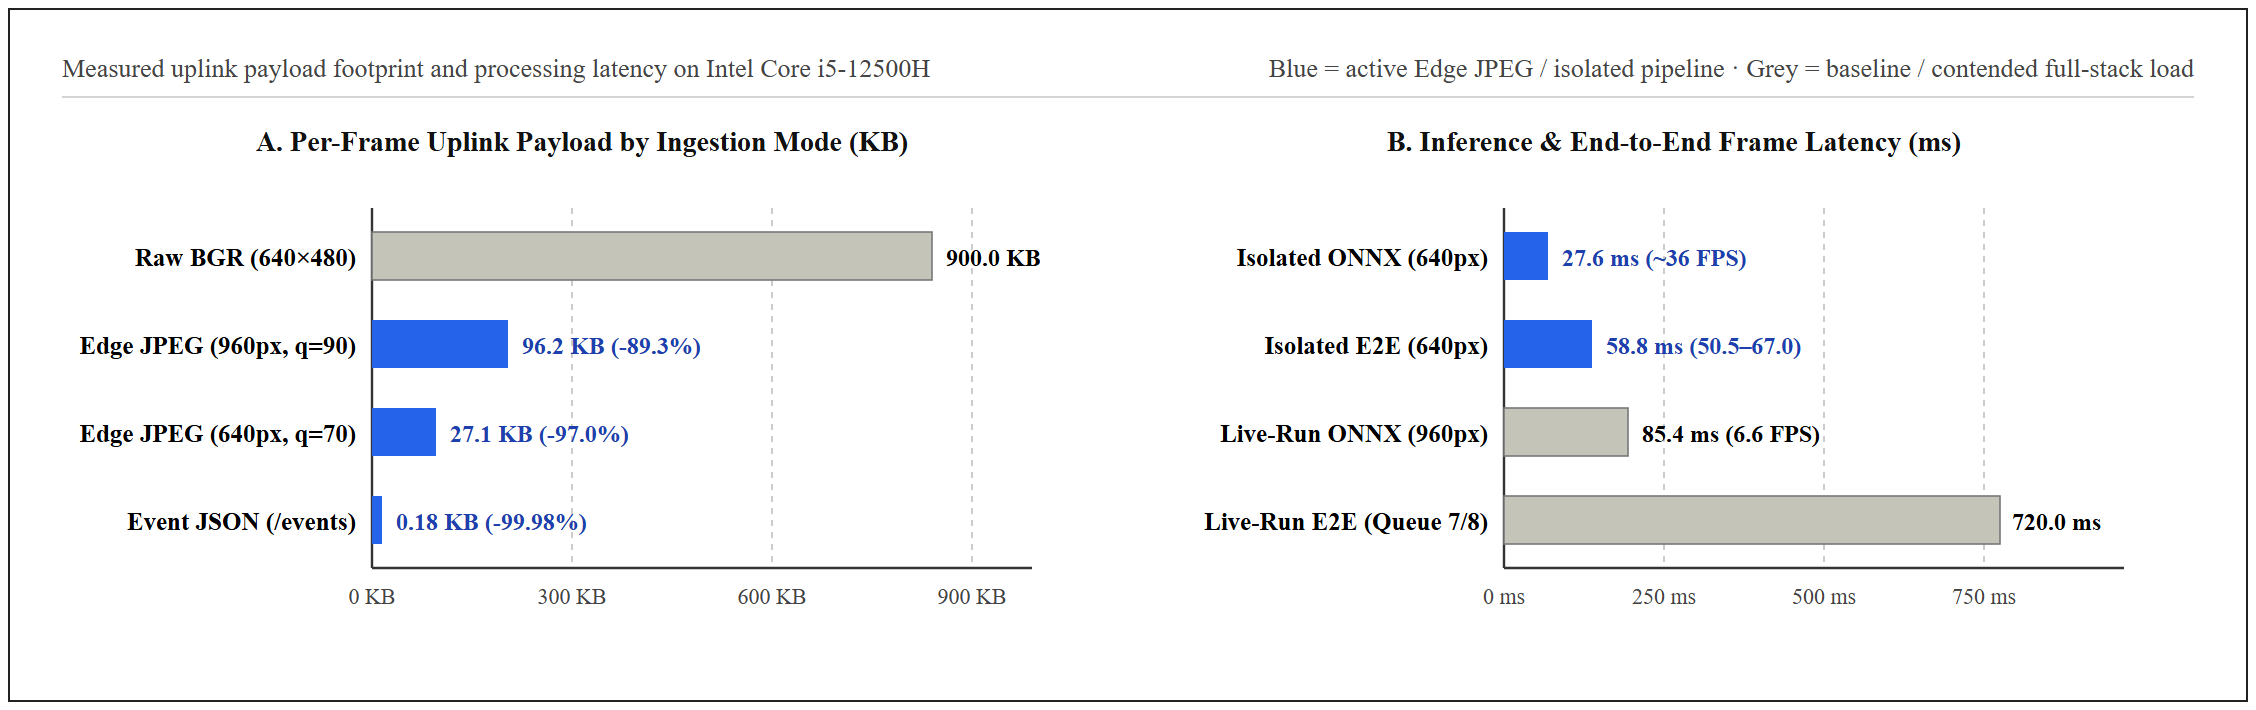
\includegraphics[width=0.98\linewidth]{figures/fig5_payload.png}
\caption{Comparison of per-frame uplink payload size across ingestion modes and isolated versus full-stack inference latency on the Intel Core i5-12500H testbed.}
\label{fig:payload}
\end{figure}

\subsection{Live run: system statistics}

Fig.~\ref{fig:analytics} was captured after the stack had been running for 4 minutes 57 seconds. Table~\ref{tab:live} and Fig.~\ref{fig:counts} reproduce the telemetry counters and queue retention metrics from the live run.

\begin{table}[H]
\centering\small
\caption{Counters read from the Analytics Console during the live run}
\label{tab:live}
\begin{tabularx}{\textwidth}{|L{4.2cm}|L{2.4cm}|Y|}
\hline
\rowcolor{black!8} \textbf{Counter} & \textbf{Value} & \textbf{Comment} \\ \hline
Total events logged & 2,605 & Debounced detection records in SQLite \\ \hline
Occupancy spikes & 74 & Cumulative database count, not only this run \\ \hline
Unexpected objects & 153 & Cumulative database count \\ \hline
Object dwell & 54 & Cumulative database count \\ \hline
Pipeline throughput & 6.6 FPS & 10-second rolling window \\ \hline
Average inference / end to end & 85.4 ms / 720 ms & Full stack on one laptop \\ \hline
Frames received & 2,859 & Server counter \\ \hline
Frames dropped & 102 & Bounded queue, drop-oldest \\ \hline
Drop rate (derived) & about 3.6\% & $102 / 2{,}859$ \\ \hline
Queue depth / average payload & 7 / 96.2 KB & 960 px at JPEG quality 90 \\ \hline
Uptime & 4 min 57 s & Server uptime \\ \hline
\end{tabularx}
\end{table}

\begin{figure}[H]
\centering
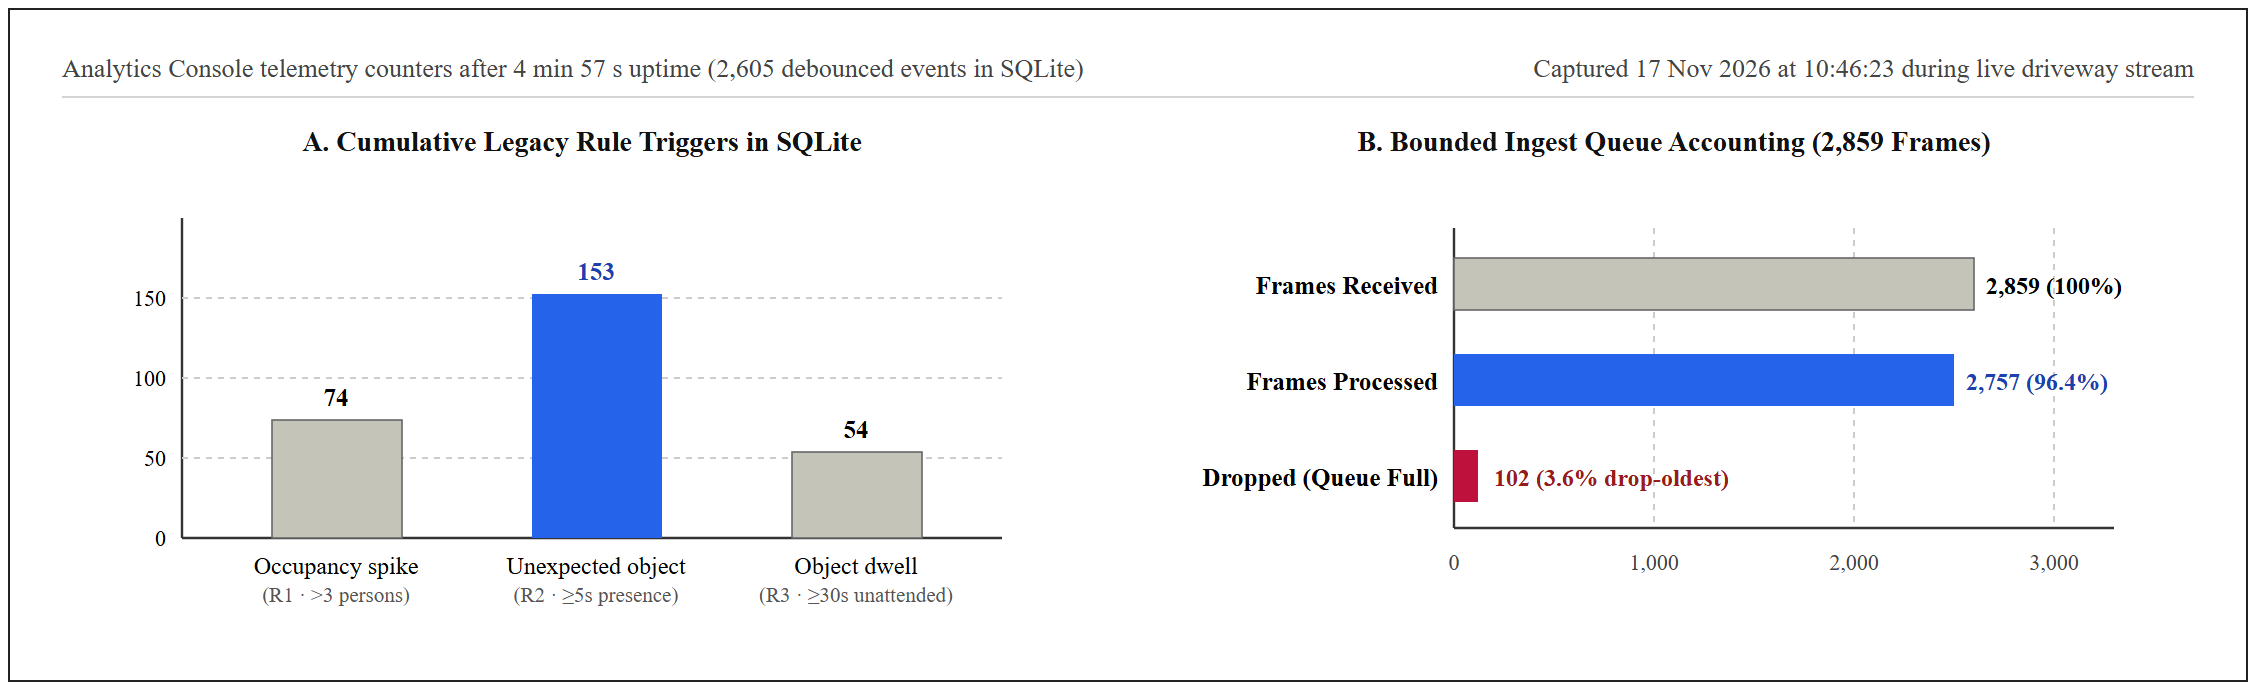
\includegraphics[width=0.98\linewidth]{figures/fig6_counts.png}
\caption{Live-run telemetry counters and ingest queue retention breakdown captured from the Analytics Console after 4 minutes 57 seconds of continuous operation.}
\label{fig:counts}
\end{figure}

\textbf{Reading the numbers.} The three rule counters come from the database's per-rule tally, which only tracks the three original public-mode rules and keeps accumulating across runs, so they say little about the single live run; the new home-mode rules are visible only in the Anomalies tab and in Telegram. Average inference time (85.4 ms) is about three times the isolated benchmark (27.6 ms), and end-to-end latency (720 ms) is far above the isolated 50--67 ms. The most plausible reasons are CPU contention from running the server, edge process, two browsers tabs, a 960 px stream and the LLM client on one machine, and queueing (depth 7 of 8). This was not profiled, so it is a hypothesis, not a finding.

\subsection{Live run: Telegram alerts}

Within about 19 seconds (10:44:21 to 10:44:39) twelve alert cards reached the phone. Table~\ref{tab:alerts} and Fig.~\ref{fig:alerttime} present the twelve alerts in chronological order, transcribed from the three mobile screenshots in Fig.~\ref{fig:telegram}.

\begin{table}[H]
\centering\small
\caption{Alerts delivered to Telegram during the live run}
\label{tab:alerts}
\begin{tabularx}{\textwidth}{|L{1.5cm}|L{1.7cm}|L{3.7cm}|L{2.2cm}|Y|}
\hline
\rowcolor{black!8} \textbf{Time} & \textbf{Level} & \textbf{Rule} & \textbf{Zone} & \textbf{Agent reason (shortened)} \\ \hline
10:44:21 & \cellcolor{yellow!20}Warning & Camera Tamper Moved & global & Sudden scene shift (0.98) \\ \hline
10:44:23 & \cellcolor{yellow!20}Warning & Night Person & global & \code{fail-open} after timeout \\ \hline
10:44:31 & \cellcolor{yellow!20}Warning & Fence Or Wall Approach & \code{fence_line} & Approaching fence at night \\ \hline
10:44:32 & \cellcolor{yellow!20}Warning & Repeat Visit Casing & \code{fence_line} & Three distinct visits \\ \hline
10:44:32 & \cellcolor{yellow!20}Warning & Repeat Visit Casing & \code{window} & Repeat visits, possible casing \\ \hline
10:44:33 & \cellcolor{red!14}Critical & Night Person & global & Two persons, confidence 0.67 \\ \hline
10:44:33 & \cellcolor{yellow!20}Warning & Fence Or Wall Approach & \code{fence_line} & Approaching fence at night \\ \hline
10:44:34 & \cellcolor{red!14}Critical & Person In Zone & \code{window} & Person at window, armed night \\ \hline
10:44:34 & \cellcolor{red!14}Critical & Fence Or Wall Approach & \code{fence_line} & Perimeter approach (escalated) \\ \hline
10:44:34 & \cellcolor{yellow!20}Warning & Person In Zone & \code{window} & Possible false positive noted \\ \hline
10:44:37 & \cellcolor{red!14}Critical & Repeat Visit Casing & \code{yard} & Three yard visits, casing \\ \hline
10:44:39 & \cellcolor{red!14}Critical & Person In Zone & \code{door} & Person at door, armed night \\ \hline
\end{tabularx}
\end{table}

\begin{figure}[H]
\centering
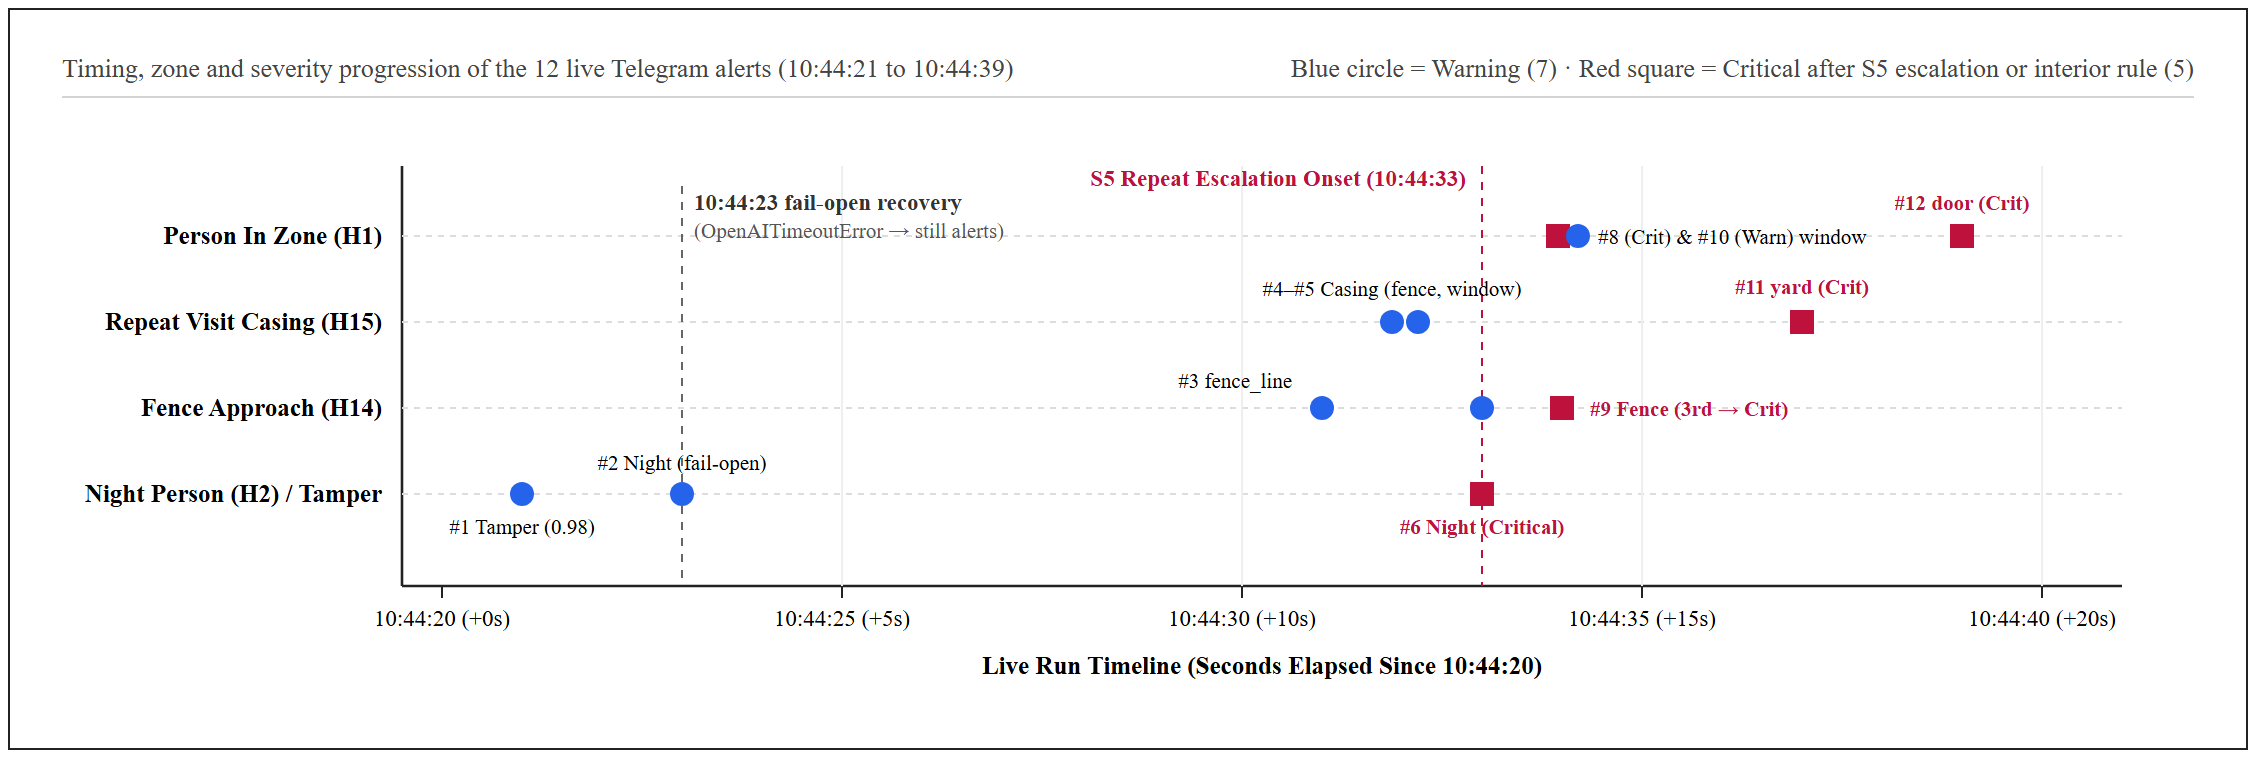
\includegraphics[width=0.98\linewidth]{figures/fig7_alert_timeline.png}
\caption{Timing and severity of the twelve alerts in Table~\ref{tab:alerts}. Warnings dominate the first ten seconds; criticals cluster later as repeat escalation takes effect.}
\label{fig:alerttime}
\end{figure}

\begin{figure}[H]
\centering
\fbox{\begin{minipage}{0.97\linewidth}
\centering
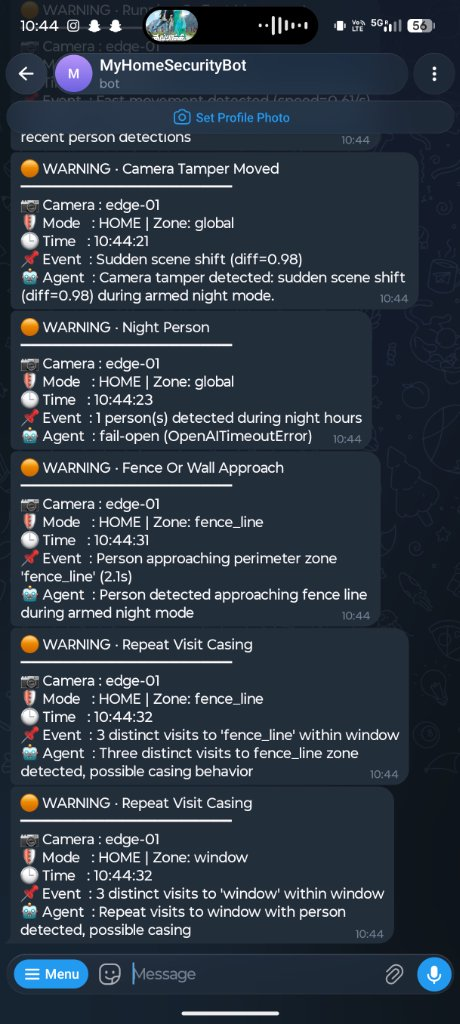
\includegraphics[height=10.2cm]{figures/telegram_1.jpg}\hfill
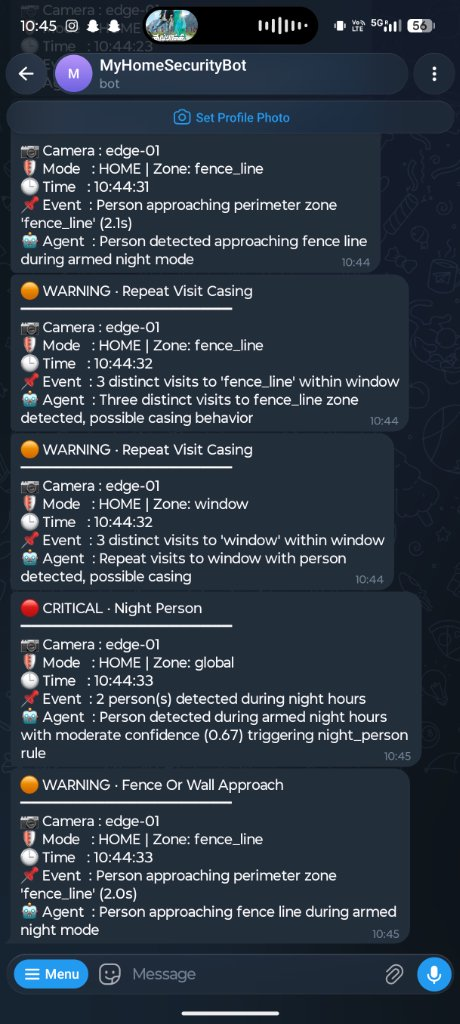
\includegraphics[height=10.2cm]{figures/telegram_2.jpg}\hfill
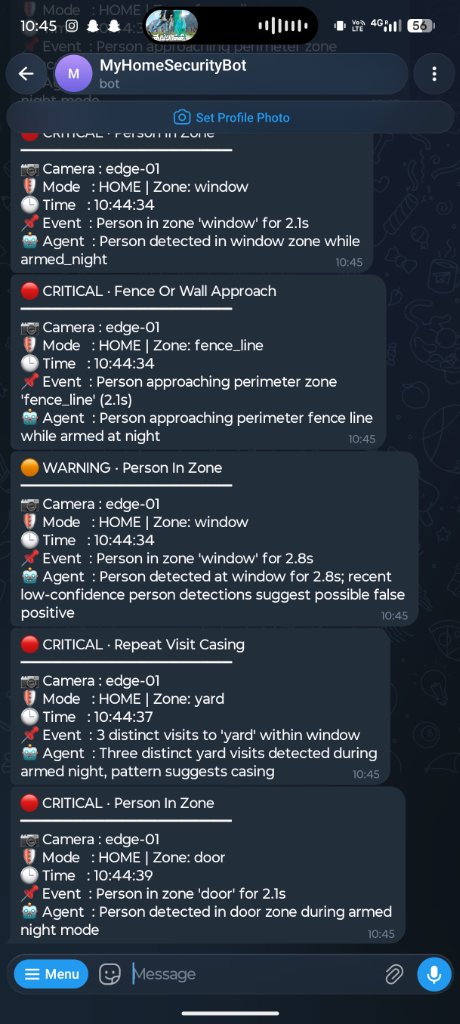
\includegraphics[height=10.2cm]{figures/telegram_3.jpg}
\end{minipage}}
\caption{Telegram alert cards received on the phone during the live run (three consecutive screenshots, 10:44--10:45). Each card shows camera, mode and zone, time, event and the agent's reason.}
\label{fig:telegram}
\end{figure}

\subsection{Automated tests}

\begin{table}[H]
\centering\small
\caption{Automated verification}
\label{tab:ieee_29}
\begin{tabularx}{\textwidth}{|L{4.2cm}|L{2.8cm}|Y|}
\hline
\rowcolor{black!8} \textbf{Check} & \textbf{Result} & \textbf{Scope} \\ \hline
\code{pytest tests -q} & \cellcolor{green!18}26 passed & Legacy rules (occupancy, unexpected, dwell, occlusion, hysteresis, cooldown), API security (401, 403, 413, 400, 422, CORS), home rules, public rules, tamper and escalation, LangGraph triage and fail-open, webhook signing, edge server routes \\ \hline
\code{scripts/eval.py} & \cellcolor{green!18}P 1.00, R 1.00 & Two self-labelled clips \\ \hline
Cloud LLM probe & \cellcolor{green!18}valid JSON, 4.5 s & One alert-style prompt \\ \hline
Frontend production build & \cellcolor{green!18}built & Vite, 29 modules \\ \hline
\end{tabularx}
\end{table}

% ---------------- 12 ----------------
\section{Discussion}

\subsection{What worked}

\begin{itemize}
  \item \textbf{The two-server split holds.} The simulated IoT edge node on \code{:8001} and the analysis server on \code{:8000} ran independently; the edge could be restarted and re-pointed without touching the server, and frames flowed over plain HTTP.
  \item \textbf{End-to-end alerting works.} A detection became a phone notification in seconds, with a readable card and a reason supplied by the language model.
  \item \textbf{Escalation and policy behave as designed.} Repeated events rose from warning to critical, and a log-only vehicle event was stored with a \code{[SUPPRESSED]} marker instead of being pushed.
  \item \textbf{Fail-open was exercised for real.} One alert shows \code{fail-open (OpenAITimeoutError)}; the alert still arrived.
\end{itemize}

\subsection{What the live run exposed}

\begin{table}[H]
\centering\small
\caption{Problems observed in the live run, likely causes and remedies}
\label{tab:ieee_30}
\begin{tabularx}{\textwidth}{|L{3.4cm}|Y|Y|}
\hline
\rowcolor{black!8} \textbf{Observation} & \textbf{Likely cause (not all verified)} & \textbf{Remedy} \\ \hline
Twelve alerts in 19 s & Many zones overlap; several rules fire on the same person; cooldown is per rule and zone & Merge duplicates, add a global alert budget, or send a digest (S7 is not implemented) \\ \hline
Person alerts on a mostly-vehicle frame & Low-confidence person detections on reflections or parked cars; one agent reason itself flags a possible false positive & Raise person threshold, require more confirmation frames, add a stationary-object filter \\ \hline
\code{Camera Tamper Moved} at 10:44:21 & Histogram changed sharply when the clip restarted or the scene changed & Reset the reference when the source changes or the clip loops \\ \hline
Repeat-visit casing within seconds & Track identities flicker; each new track id counts as a distinct visit & Merge tracks that reappear in the same place, lengthen the visit window \\ \hline
Zones do not match the footage & Default polygons were written for a generic layout, not for this camera & Calibrate polygons per camera in the console \\ \hline
Inference 85.4 ms, end to end 720 ms & Single-laptop contention and queueing (hypothesis) & Profile; run edge and server on separate machines \\ \hline
One \code{fail-open} & LLM request timed out at 20 s & Retry once, raise timeout, or cache similar decisions \\ \hline
\end{tabularx}
\end{table}

\subsection{Is the alert volume acceptable?}

Not yet, and the report states that plainly. A homeowner who receives a dozen cards in twenty seconds will mute the bot, which defeats the purpose. The causes are mostly configuration and tuning (zones not calibrated to the footage, overlapping zones, generous casing logic) rather than a flaw in the architecture. The architecture does provide the right hooks for fixing it: a policy per rule, a severity escalation stage, and a triage agent that can suppress \code{review} rules. What is missing is a global rate limit and a digest, both listed as future work.

\subsection{Is the LLM adding value?}

The reasons attached to alerts are readable and sometimes useful: one card says that recent low-confidence person detections suggest a possible false positive. However, in this run the model confirmed almost every alert it saw, so there is no evidence yet that it reduced false positives. To show that, the system would need labelled alert data and a comparison with and without the agent. This is an honest gap, not a result.

% ---------------- 13 ----------------
\section{Deployment and Operation}

\subsection{Start-up order}

Five terminals are used. Hermes can already be running from an earlier session, in which case only four are needed.

\begin{table}[H]
\centering\small
\caption{Commands to run the full stack (each in its own terminal, from the project folder)}
\label{tab:ieee_31}
\begin{tabularx}{\textwidth}{|r|L{3.2cm}|Y|}
\hline
\rowcolor{black!8} \textbf{\#} & \textbf{Process} & \textbf{Command} \\ \hline
1 & Hermes gateway & \texttt{hermes gateway run} (from the Hermes install folder) \\ \hline
2 & Analysis server \code{:8000} & \texttt{.venv\textbackslash Scripts\textbackslash python.exe -m uvicorn server.app:app --port 8000} \\ \hline
3 & Simulated IoT edge \code{:8001} & \texttt{.venv\textbackslash Scripts\textbackslash python.exe -m uvicorn edge.edge\_server:app --port 8001} \\ \hline
4 & Analytics Console \code{:5173} & \code{cd frontend} then \code{npm run dev:analytics} \\ \hline
5 & Edge Control Deck \code{:5174} & \code{cd frontend} then \code{npm run dev:edge} \\ \hline
\end{tabularx}
\end{table}

\subsection{Deployment variants}

\begin{table}[H]
\centering\small
\caption{Deployment variants}
\label{tab:ieee_32}
\begin{tabularx}{\textwidth}{|L{3.4cm}|Y|}
\hline
\rowcolor{black!8} \textbf{Variant} & \textbf{How} \\ \hline
All on one laptop (used here) & Five terminals as above; edge simulated as a separate process \\ \hline
Two machines on a LAN & Server started with a host binding and an API key; edge machine sets \code{AIIOT_SERVER_URL} to the server address \\ \hline
Real IoT device (future) & Run \code{edge/} on a Raspberry Pi 4 with a USB webcam; server unchanged \\ \hline
Embedded edge (legacy) & \code{EMBEDDED_EDGE=1} runs the emitter inside the server; not used in this report \\ \hline
Edge inference (future) & Move the detector onto the device and post only JSON to \code{/events} \\ \hline
\end{tabularx}
\end{table}

\subsection{Troubleshooting notes}

\begin{table}[H]
\centering\small
\caption{Problems met while running the system}
\label{tab:ieee_33}
\begin{tabularx}{\textwidth}{|L{3.8cm}|Y|}
\hline
\rowcolor{black!8} \textbf{Symptom} & \textbf{Explanation and fix} \\ \hline
Consoles say backend unreachable & The consoles started before the backends finished loading; refresh once both ports respond \\ \hline
Repeated \code{WinError 10054} tracebacks & Harmless Windows asyncio noise when the browser closes a polled keep-alive socket; a handler that ignores this one error was added to both servers \\ \hline
\code{npm} blocked in PowerShell & Script execution policy blocks \code{npm.ps1}; use \code{npm.cmd} or a normal command prompt \\ \hline
Telegram receives nothing & Hermes gateway not running; check port 8644 and start it in a normal window \\ \hline
Two emitters on one device id & An old embedded or CLI emitter was still running; stop all but one \\ \hline
\code{401} when binding to all interfaces & By design: unauthenticated posts are refused unless an API key is set \\ \hline
\end{tabularx}
\end{table}

% ---------------- 14 ----------------
\section{Testing and Verification}

\begin{table}[H]
\centering\small
\caption{Test inventory}
\label{tab:ieee_34}
\begin{tabularx}{\textwidth}{|L{4.6cm}|L{1.4cm}|Y|}
\hline
\rowcolor{black!8} \textbf{Group} & \textbf{Tests} & \textbf{What is checked} \\ \hline
Legacy public rules & 10 & Occupancy spike, unexpected object, dwell, owner reset, passer-by, nudge, occlusion, two bags, hysteresis, cooldown \\ \hline
API and ingest & 1 & Frames and events, 400 and 413 and 202 paths, health \\ \hline
Security & 7 & Missing key, wrong key, content-length guard, oversize JPEG, config bounds, bad source, CORS \\ \hline
Client behaviour & 1 & API key header sent by simulator \\ \hline
Home rules & 2 & Zones, night, loiter, pets, package left and taken, person down \\ \hline
Public rules & 1 & Sudden dispersal and vehicle in pedestrian zone \\ \hline
Camera health & 1 & Blocked camera and repeat escalation \\ \hline
Agent & 1 & Confirm, suppress and fail-open paths \\ \hline
Alerts & 1 & Webhook signature header \\ \hline
Edge server & 1 & Health and status routes of the separate edge process \\ \hline
\textbf{Total} & \textbf{26} & All passing \\ \hline
\end{tabularx}
\end{table}

\textbf{What is not tested.} The live behaviour with the full stack, the console interactions in a browser, the LLM's quality, and the physical-device path are not covered by automated tests. The live run in Section~\ref{sec:results} is a manual demonstration.

% ---------------- 15 ----------------
\section{Limitations}\label{sec:limits}

\begin{itemize}
  \item \textbf{The IoT device is simulated.} The edge node is a separate process reading video files, not a Raspberry Pi with a camera; hardware behaviour (power, thermals, Wi-Fi loss, camera drivers) is untested.
  \item \textbf{Detector classes.} COCO-80 has no parcel, fall-pose, face, fire or weapon classes. Parcels are proxied by bags, and \code{person_down} is an aspect-ratio heuristic that a person lying on a sofa could trigger.
  \item \textbf{Unimplemented catalogue items.} S4 (low-visibility mode), S7 (quiet-hours digest) and P14 (illegal parking) were designed but not built.
  \item \textbf{Playback timing.} Clips at 30 or 60 FPS are read one frame per tick at 5 FPS, so they play in slow motion; thresholds are in emission seconds.
  \item \textbf{Zone calibration.} Polygons and thresholds are starting guesses; none has been tuned against labelled footage.
  \item \textbf{Evaluation.} The offline score uses two self-labelled clips. No independent accuracy figure is claimed.
  \item \textbf{LLM value is unproven.} No with/without comparison has been run, and the agent depends on a cloud service whose latency varied between 4.5 s and a timeout.
  \item \textbf{Database counters.} The statistics endpoint tallies only three legacy rule names and accumulates over runs.
\end{itemize}

% ---------------- 16 ----------------
\section{Future Work}

\begin{enumerate}
  \item Run the edge process on a real Raspberry Pi 4 with a USB webcam and measure uplink, frame loss and thermal behaviour.
  \item Label the four security-camera clips and the Intel clips, extend \code{eval.py} to per-rule precision and recall, and use the numbers to tune thresholds.
  \item Add a global alert budget and a digest (S7), merge duplicate alerts, and reset the tamper reference when the source changes.
  \item Add a zone-drawing tool to the Edge Control Deck so polygons are calibrated on the first frame of each camera.
  \item Compare alert precision with and without the triage agent on labelled data, and try a smaller local model for privacy and latency.
  \item Add a pose or fall model and a parcel class (by fine-tuning) to retire the heuristic rules; implement P14 and S4.
  \item Add authentication to the edge control API and bind the Hermes webhook to loopback.
  \item Install the Hermes gateway as a scheduled service so Telegram survives reboots.
\end{enumerate}

% ---------------- 17 ----------------
\section{Conclusion}

The project shows that a home or public-space CCTV analyser can be built with local video processing, two cleanly separated servers, a domain-aware rule engine and a text-only language-model triage stage, and that its alerts can reach a phone in structured form within seconds. The simulated IoT edge node (\code{:8001}) and the analysis server (\code{:8000}) cooperate only over HTTP, which is the boundary a real device would use. JPEG encoding reduces uplink traffic by about 97\%, local inference runs at tens of milliseconds, and the automated suite of 26 tests passes. The live run is equally important for what it exposed: alert bursts, an uncalibrated zone layout, a tamper flag at the video loop and an LLM timeout. Each is understood, each has a remedy, and none is hidden. The next step is to move the edge process onto real hardware and to measure alert quality on labelled footage.

\begin{center}
\textbf{\large Keep the video local. Let the agent explain the alert.}
\end{center}

% ---------------- References ----------------
\section*{References}
\addcontentsline{toc}{section}{References}

\begin{table}[H]
\centering\small
\caption{References and software components used}
\label{tab:ieee_35}
\begin{tabularx}{\textwidth}{|r|Y|Y|}
\hline
\rowcolor{black!8} \textbf{\#} & \textbf{Source} & \textbf{Used for} \\ \hline
01 & Ultralytics YOLO26 (NMS-free ONNX export) & Object detection model \\ \hline
02 & ONNX Runtime & CPU inference without PyTorch \\ \hline
03 & FastAPI, Uvicorn and Pydantic & Ingest API, edge control API, validation \\ \hline
04 & OpenCV and NumPy & Capture, letterboxing, polygon tests, annotation \\ \hline
05 & LangChain and LangGraph & Four-node triage workflow \\ \hline
06 & NVIDIA cloud inference endpoint (OpenAI-compatible) & Language model for triage \\ \hline
07 & Nous Research Hermes Agent v0.23.1 & Webhook gateway and Telegram delivery \\ \hline
08 & Telegram Bot API & Phone notifications \\ \hline
09 & Intel IoT DevKit sample videos (GitHub) & Public demonstration clips \\ \hline
10 & Open GitHub repository of security-camera clips (Security-Camera-w-AI) & Four security-camera clips \\ \hline
11 & React, Vite and headless Edge HTML/CSS renderer & Web consoles and high-DPI report diagrams \\ \hline
\end{tabularx}
\end{table}

% ---------------- Appendices ----------------
\clearpage
\appendix
\section{Application Programming Interfaces}

\begin{table}[H]
\centering\small
\caption{Analysis server endpoints (port 8000)}
\label{tab:ieee_36}
\begin{tabularx}{\textwidth}{|L{3.4cm}|L{1.7cm}|Y|}
\hline
\rowcolor{black!8} \textbf{Endpoint} & \textbf{Method} & \textbf{Purpose} \\ \hline
\code{/frames} & POST & Ingest a JPEG with device id, timestamp, sequence, source kind \\ \hline
\code{/events} & POST, GET & Inject a detection event; list recent events \\ \hline
\code{/anomalies} & GET & Recent anomalies including suppressed records \\ \hline
\code{/frames/latest} & GET & Latest annotated JPEG \\ \hline
\code{/devices} & GET & Connected devices and counters \\ \hline
\code{/stats} & GET & KPIs, throughput, latency, drop counters \\ \hline
\code{/health} & GET & Worker and model status; 503 when degraded \\ \hline
\code{/mode} & GET, POST & Read or switch mode and arming \\ \hline
\end{tabularx}
\end{table}

\begin{table}[H]
\centering\small
\caption{SQLite tables (WAL mode)}
\label{tab:ieee_37}
\begin{tabularx}{\textwidth}{|L{3.0cm}|Y|}
\hline
\rowcolor{black!8} \textbf{Table} & \textbf{Columns} \\ \hline
\code{events} & id, ts, device\_id, source, object\_class, count, avg\_conf \\ \hline
\code{anomalies} & id, ts, device\_id, rule, detail, severity \\ \hline
\code{frame_metrics} & id, ts, device\_id, frame\_bytes, inference\_ms, e2e\_ms \\ \hline
\end{tabularx}
\end{table}

\section{Configuration Excerpt}

The following excerpt of \code{config.yaml} shows the settings that most affect behaviour.

\begin{small}
\begin{verbatim}
edge:    {device_id: edge-01, fps: 5, width: 960, jpeg_quality: 90}
server:  {queue_size: 8, conf: 0.4, conf_stay: 0.3, debounce_seconds: 2,
          class_thresholds: {person: 0.40, backpack: 0.30, handbag: 0.30,
                             suitcase: 0.30, knife: 0.35, scissors: 0.35}}
mode: public            # public | home  (switchable via POST /mode)
arming: armed_night     # disarmed | armed_home | armed_night | armed_away
rules:   {person_threshold: 3, unexpected_seconds: 5, dwell_seconds: 30,
          owner_radius: 0.20, track_timeout: 15, cooldown_seconds: 10,
          offline_seconds: 30, repeat_escalation_count: 3}
home:    {night: {start: "22:00", end: "06:00"},
          ignore_classes: [dog, cat], loiter_seconds: 20,
          zones: {door, window, yard, driveway, fence_line, pool}}
public:  {capacity_limit: 20, loiter_s: 120, running_speed: 0.35,
          operating_hours: {start: "08:00", end: "22:00"},
          zones: {restricted, pedestrian, no_parking, no_wheels, queue}}
agent:   {enabled: true, provider: nvidia, timeout_s: 20.0,
          model: nvidia/nemotron-3-ultra-550b-a55b}
\end{verbatim}
\end{small}

\section{Repository Layout}

\begin{table}[H]
\centering\small
\caption{Project layout}
\label{tab:ieee_38}
\begin{tabularx}{\textwidth}{|L{3.4cm}|Y|}
\hline
\rowcolor{black!8} \textbf{Path} & \textbf{Contents} \\ \hline
\code{edge/} & \code{capture.py}, \code{controller.py}, \code{edge_server.py}, \code{edge_client.py} \\ \hline
\code{server/} & \code{app.py}, \code{worker.py}, \code{pipeline.py}, \code{detector.py}, \code{tracker.py}, \code{rules.py}, \code{agent.py}, \code{alerts.py}, \code{db.py} \\ \hline
\code{frontend/src/} & \code{AnalyticsApp.jsx}, \code{EdgeEmitterApp.jsx}, \code{components/ConsoleShell.jsx}, \code{styles.css} \\ \hline
\code{scripts/} & \code{eval.py}, \code{simulator.py}, \code{export_model.py} \\ \hline
\code{tests/} & \code{test_rules.py} (26 tests) \\ \hline
\code{data/} & Demonstration video clips and state file \\ \hline
\code{report/} & This report (\code{main.tex}, \code{figures/}) \\ \hline
\end{tabularx}
\end{table}

\end{document}
